%--------------------------------------
% Create title frame
\titleframe

%--------------------------------------
% Table of contents
\begin{frame}{Overview}
  \setbeamertemplate{section in toc}[sections numbered]
  \tableofcontents[hideallsubsections]
\end{frame}



%--------------------------------------

\begin{frame}[allowframebreaks]{Que sont les régimes transitoires?}
Dans un circuit comportant des éléments linéaires et invariants R, L, C et des sources indépendantes d'énergie, lorsque des variations se produisent (changement de topologie ou sources d'alimentations variables) les grandeurs électriques fluctuent, il y a un \alert{régime transitoire}.

Lorsques les variations de courant ou de tension sont dues à des variations brusques des tensions ou des courants des sources d'alimentation, on parle de \alert{réponse forcée}.

Inductances et condensateurs sont des éléments capables d'emmagasiner une certaine quantité d'énergie (magnétostatique ou électrostatique).
La \alert{réponse libre} correspond aux phénomènes survenant lorsque cette énergie, emmagasinée dans un élément, est subitement relachée et dissipée dans un circuit résistif.

Lorsque le régime transitoire se termine, le circuit atteint un \alert{régime permanent}.
\end{frame}


\section{Circuit RC}

\begin{frame}{Circuit RC}
\begin{center}
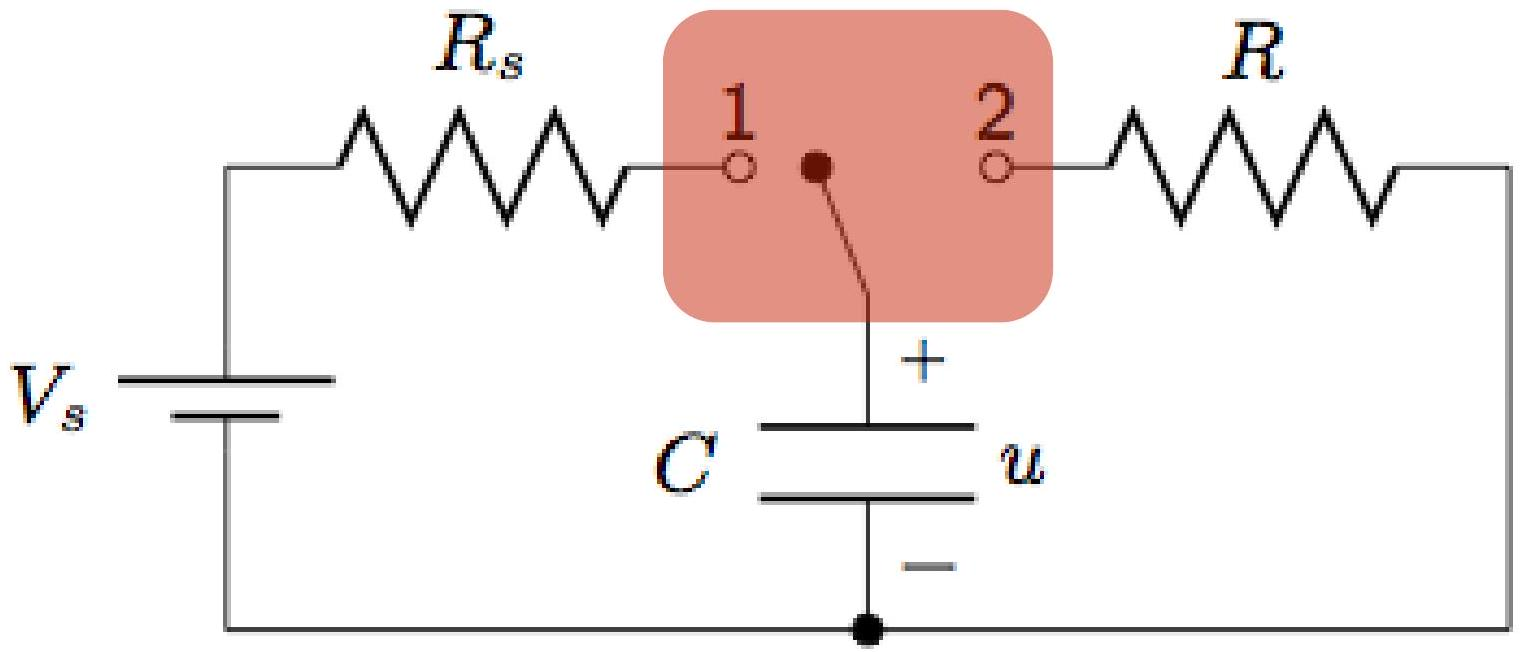
\includegraphics[width=0.4\textwidth]{images/0aae1f8e-05fc-4834-a308-b46d85861175-51_652_1520_543_937}
\end{center}

\begin{enumerate}
  \item Interrupteur en position 1 : \textbf{réponse forcée}, charge du condensateur. Porté finalement au potentiel $V_{s}$, il emmagasine une énergie
\end{enumerate}
$$
w_{C}=\frac{1}{2} C V_{s}^{2}
$$

\begin{enumerate}
  \setcounter{enumi}{1}
  \item Interrupteur en position 2 : \textbf{réponse libre}, décharge du condensateur, l'énergie emmagasinée dans $C$ est progressivement relachée et dissipée dans la résistance.
\end{enumerate}

\end{frame}


\begin{frame}[allowframebreaks]{Charge du condensateur : réponse forcée}

On suppose le condensateur initialement relaxé (il ne porte aucune énergie). 
En $t=0$, l'interrupteur bascule en position 1.\\[5mm]
\begin{columns}
  \begin{column}{0.45\textwidth}
  	(Partie de gauche du circuit)\\
	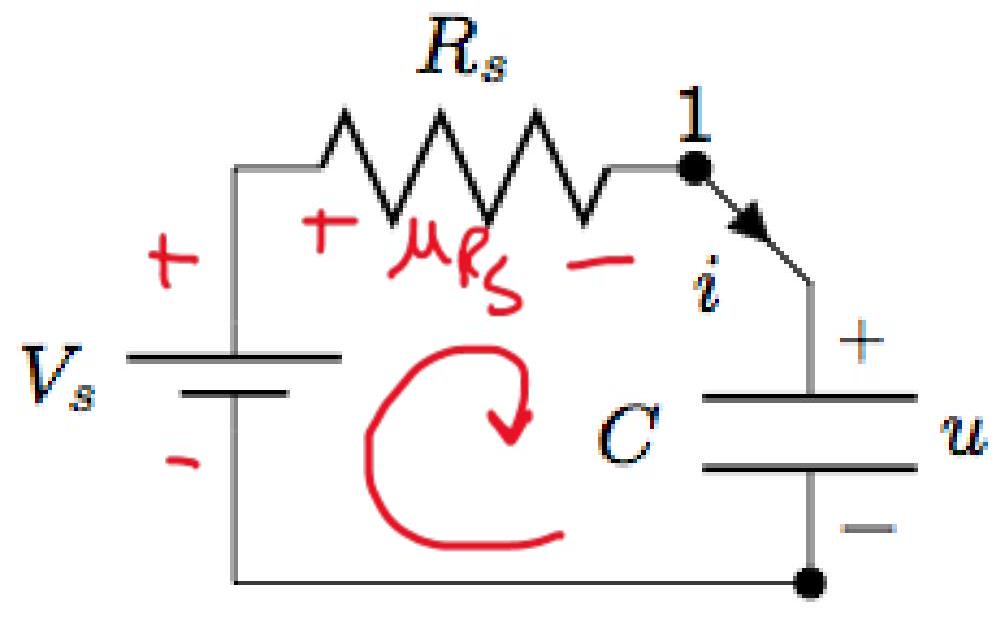
\includegraphics[width=0.5\textwidth]{images/0aae1f8e-05fc-4834-a308-b46d85861175-52_617_1006_903_320}
  \end{column}
  \begin{column}{0.45\textwidth}
	SLK : $V_{s}-u_{R_{S}}-u=0$\\
	Ohm : $u_{R_{S}}=R_{S} i$\\
	Condensateur : $i=C \frac{d u}{d t}$\\
	$\Rightarrow V_{s}-R_{s} C \frac{d u}{d t}-u=0$
  \end{column}
\end{columns}

On a donc, en $t<0$ avec $u(t)=0$:
$$\frac{d u}{d t}+\frac{u}{C R_{s}}=\frac{V_{s}}{C R_{s}}$$
Dont la solution est du type
$$u(t)=K e^{-t /\tau_{s}}+V_{s}$$

Pour déterminer la constante $K$ :
\begin{itemize}
  \item $u(0-)=0 \quad \rightarrow \quad u(0+)=0$ (continuité de $u) \rightarrow K=-V_{s}$
\end{itemize}
Donc 
$$
\boxed{u(t)=V_{s}\left(1-e^{-t / \tau_{s}}\right), \quad t>0}
$$

La grandeur $\boxed{\tau_{s}=R_{s} C}$ est la \alert{constante de temps} qui caractérise la vitesse de la charge.

\end{frame}

\begin{frame}{Régime permanent, régime transitoire}
$$
\begin{aligned}
u(t) & =V_{s}-V_{s} e^{-t / \tau_{s}} \\
& =\text { régime permanent (DC) }+ \text { régime transitoire }
\end{aligned}
$$

\begin{center}
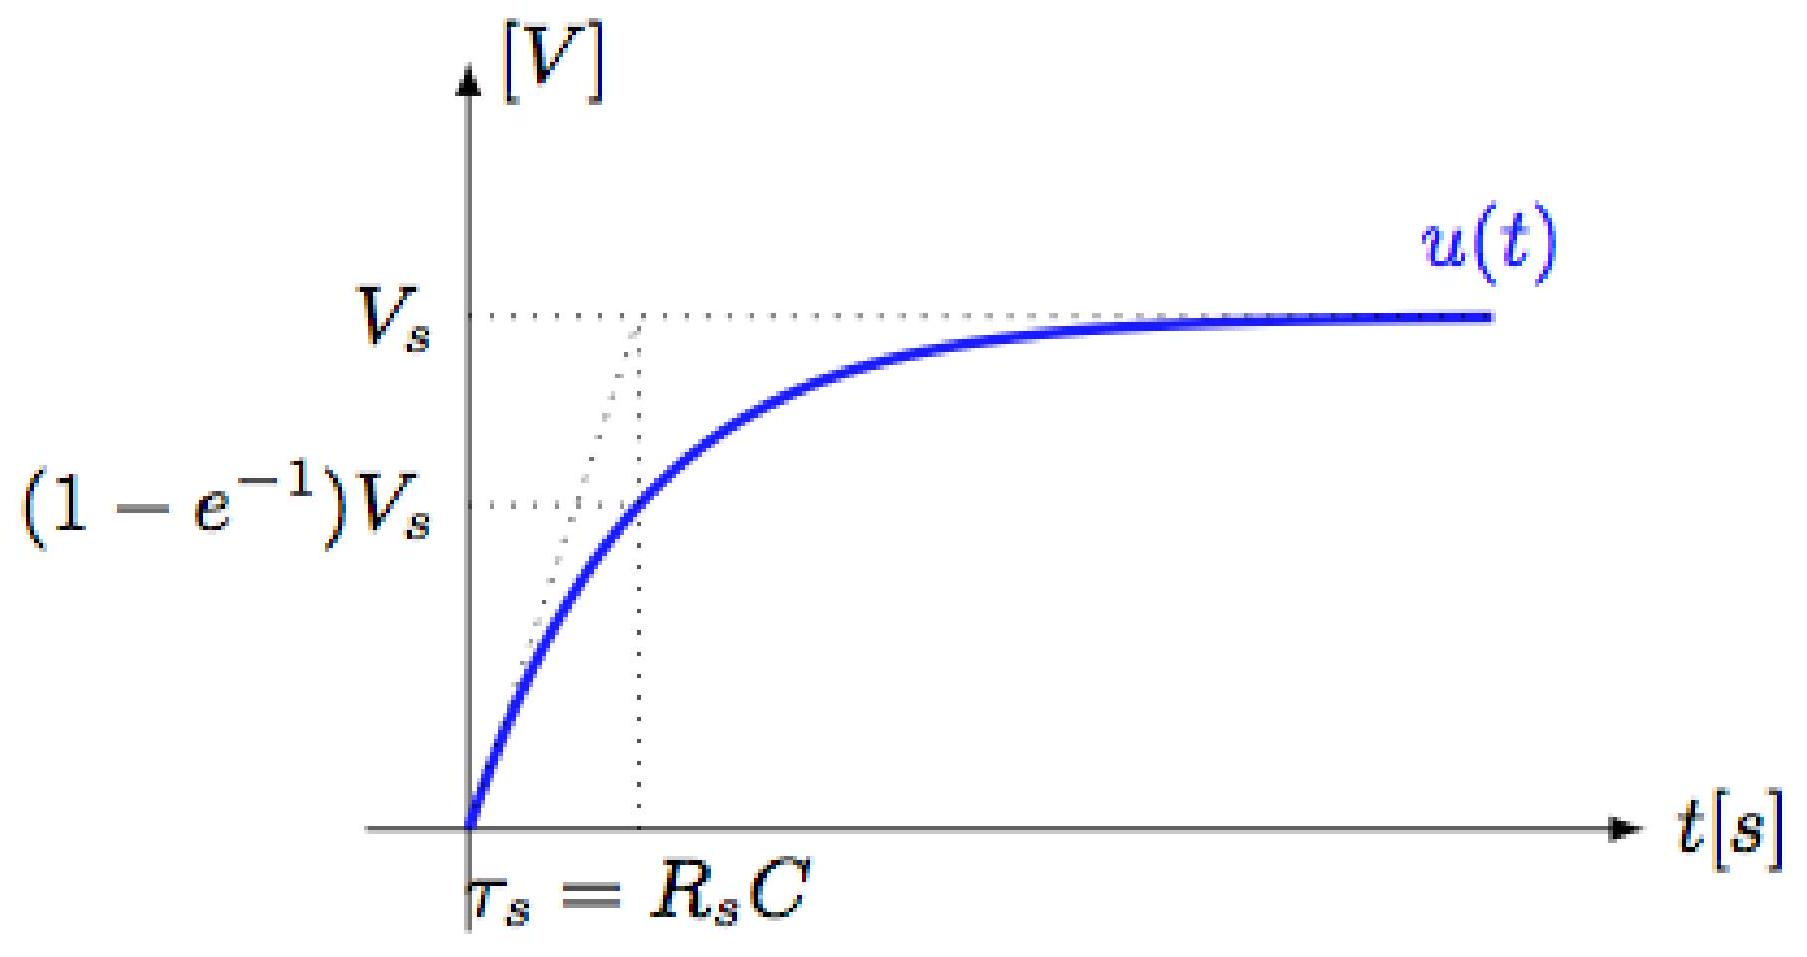
\includegraphics[width=0.4\textwidth]{images/0aae1f8e-05fc-4834-a308-b46d85861175-53_957_1807_937_786}
\end{center}

Au-delà de $5 \tau_{s}$, le régime transitoire est négligeable et $u(t) \simeq V_{s}$

\end{frame}

\begin{frame}{Courant de charge}
$$
\begin{aligned}
i(t) & =C \frac{d u}{d t}=\frac{V_{s}}{R_{s}} e^{-t / \tau_{s}} \\
i(0-) & =0, \quad i(0+)=\frac{V_{s}}{R_{s}}=i_{0}
\end{aligned}
$$

\begin{center}
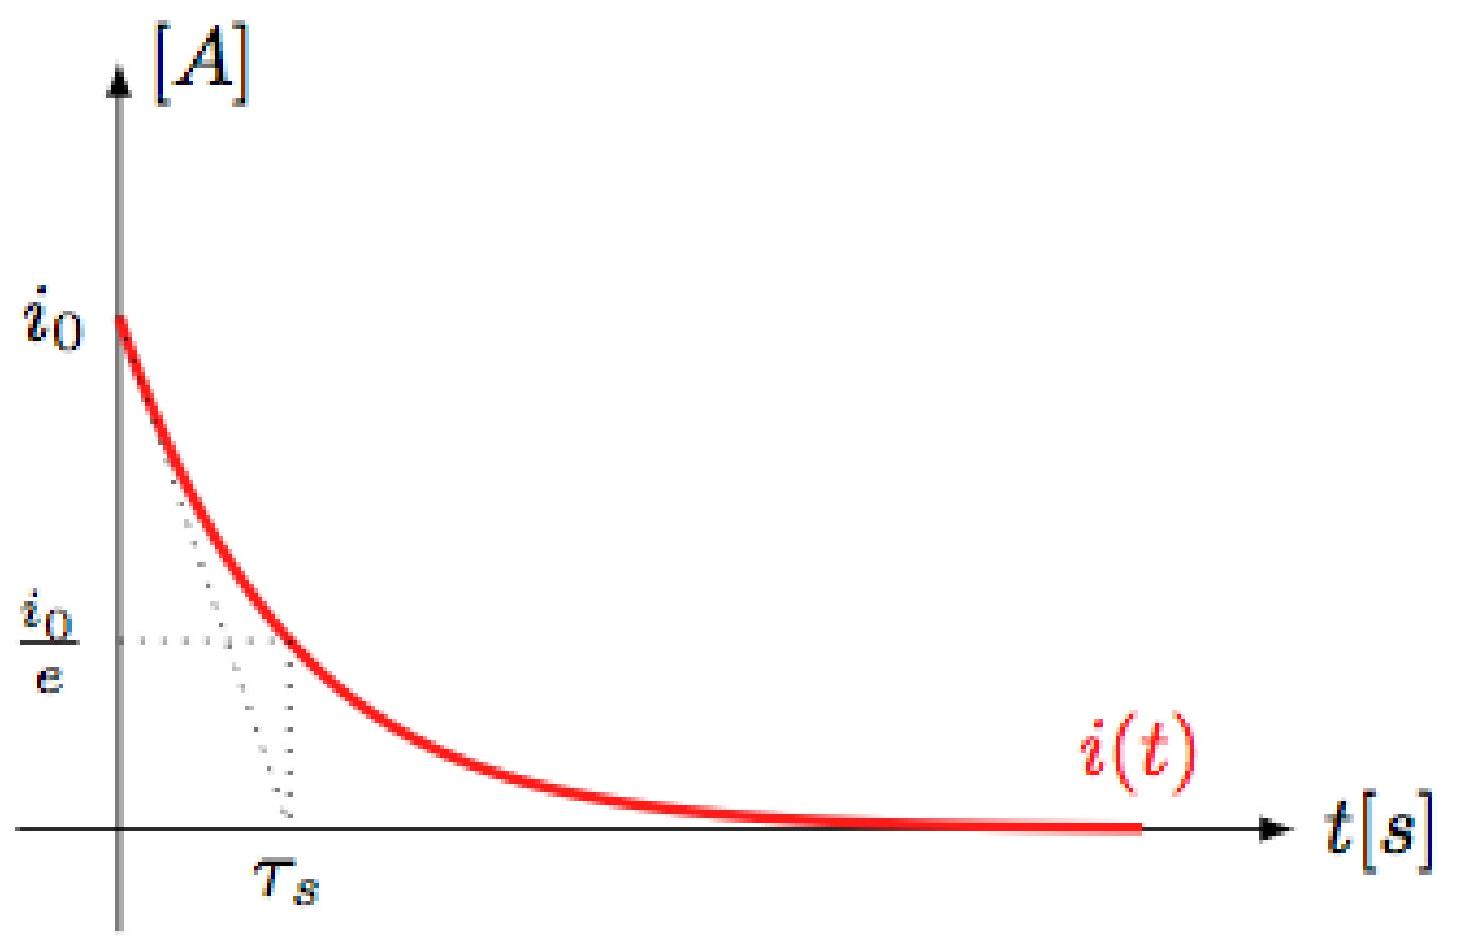
\includegraphics[width=0.4\textwidth]{images/0aae1f8e-05fc-4834-a308-b46d85861175-54_952_1458_1073_975}
\end{center}

\end{frame}

\begin{frame}{Bilan énergétique de l'opération de charge}
\begin{enumerate}
  \item Energie dissipée dans la résistance $R_{s}$ :
  $$
  p_{R}(t)=\frac{V_{s}^{2}}{R_{s}} e^{-2 t / R_{s} C}, \quad w_{R}(\infty)=\int_{0}^{\infty} p_{R}(t) d t=\frac{V_{s}^{2} C}{2}
  $$
  Indépendant de $R_{s}$ !!\\
  \item Energie emmagasinée dans le condensateur :
  
  $$
  p_{C}(t)=\frac{V_{s}^{2}}{R_{s}} e^{-t / R_{s} C}\left(1-e^{-t / R_{s} C}\right), \quad w_{C}(\infty)=\int_{0}^{\infty} p_{C}(t) d t=\frac{V_{s}^{2} C}{2}=w_{R}!
  $$
  \item Energie fournie par la pile :
  $$
  w_{V}=w_{R}+w_{C}=V_{s} \int_{0}^{\infty} i(t) d t=V_{s}^{2} C
  $$
  \item Rendement de l'opération de charge : $\eta=\frac{w_{C}}{w_{V}}=0.5$, \alert{indépendant} de $R_{s}$ et de $C$ !
\end{enumerate}





\end{frame}

\begin{frame}{Réponse libre}
Après un temps suffisamment long (supposé $\infty, u(t)=V_{s}$ ), l'interrupteur bascule en position 2. Soit $t=0$ cet instant.\\[5mm]
\begin{columns}
  \begin{column}{0.45\textwidth}
	(Partie de droite du circuit)\\
	\begin{center}
		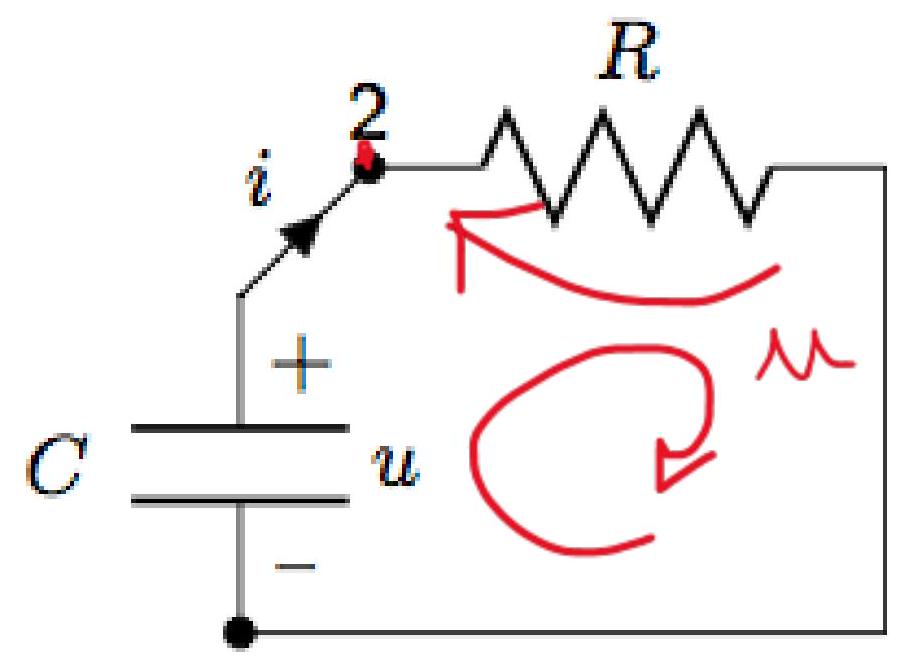
\includegraphics[width=0.4\textwidth]{images/0aae1f8e-05fc-4834-a308-b46d85861175-56_666_899_883_534}
	\end{center}
  \end{column}
  \begin{column}{0.45\textwidth}
	$$
	\begin{gathered}
	C \frac{d u}{d t}+\frac{u}{R}=0 \\
	\frac{d u}{u}=-\frac{d t}{R C} \\
	u(t)={K e^{-t / R C}}=K e^{-t / \tau}
	\end{gathered}
	$$
  \end{column}
\end{columns}


Détermination de la constante K :
\begin{itemize}
  \item $u(0-)=V_{s} \quad \rightarrow \quad u(0+)=V_{s}($ continuité de $u) \rightarrow K=V_{s}$
\end{itemize}
Donc 
$\boxed{u(t)=V_{s} e^{-t / R C}, \quad i(t)=\frac{V_{s}}{R} e^{-t / R C}, \quad t>0}$

\end{frame}

\begin{frame}{Constante de temps}
	\begin{columns}
  \begin{column}{0.45\textwidth}
	\begin{center}
	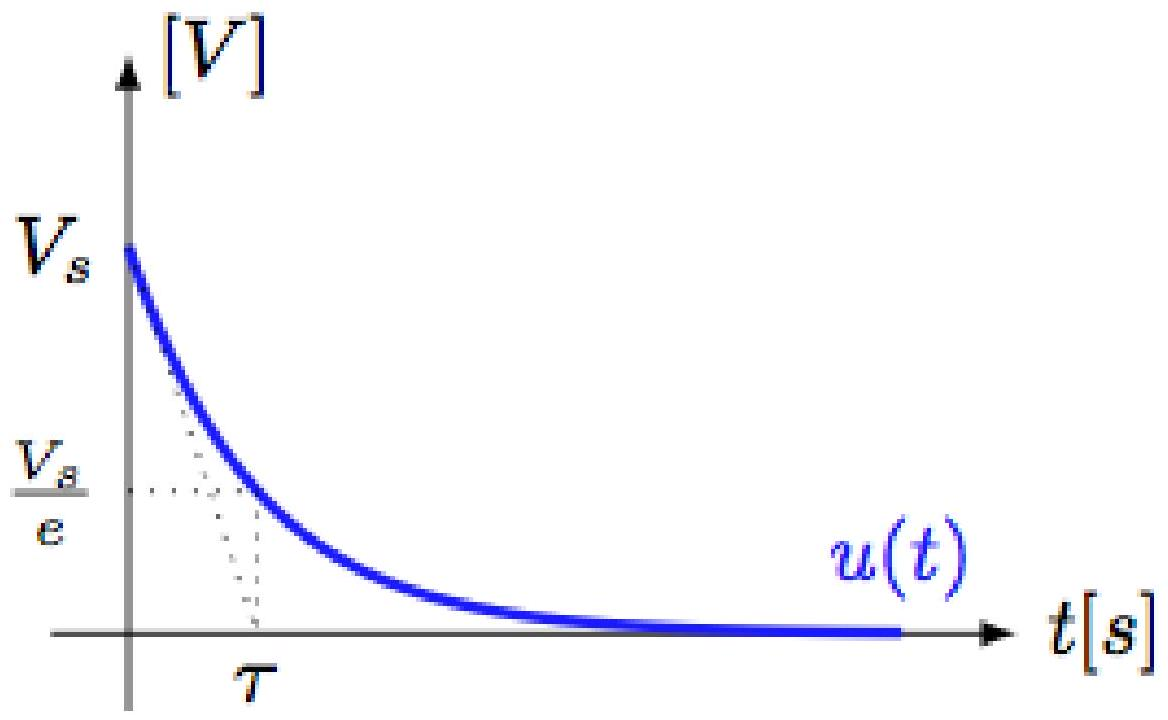
\includegraphics[width=0.6\textwidth]{images/0aae1f8e-05fc-4834-a308-b46d85861175-57_720_1168_503_303}
	\end{center}  
  \end{column}
  \begin{column}{0.45\textwidth}
$\boxed{\tau=R C}$
$$
\begin{aligned}
& u(t)=V_{s} e^{-t / \tau} \\
& i(t)=\frac{V_{s}}{R} e^{-t / \tau}
\end{aligned}
$$
  \end{column}
\end{columns}

\begin{itemize}
  \item après $\tau$ s, la tension est réduite d'un facteur $e\left(\simeq 0.368 V_{s}\right)$
  \item après $5 \tau $ s, la tension est réduite à moins de $1 \%$ de sa valeur initiale
  \item $\frac{V_{s}}{\tau}$ est la pente de la tangente en $t=0$ de la courbe $u(t)$
  \item $-\frac{1}{\tau}$, la racine du polynôme caractéristique, est appelée la fréquence naturelle du circuit
\end{itemize}

\end{frame}

\begin{frame}{Energie dissipée dans la résistance}
Puissance absorbée par la résistance:
$$
p(t)=R i^{2}(t)=\frac{V_{s}^{2}}{R} e^{-2 t / \tau}>0 \quad \forall t
$$

Energie dissipée dans l'intervalle $[0, t]$ :
$$
\begin{gathered}
w(t)=\int_{0}^{t} p(x) d x=\int_{0}^{t} \frac{V_{s}^{2}}{R} e^{-2 x / \tau} d x=\frac{1}{2} C V_{s}^{2}\left(1-e^{-2 t / \tau}\right) \\
\lim _{t \rightarrow \infty} w(t)=\frac{1}{2} C V_{s}^{2}
\end{gathered}
$$

L'énergie initialement emmagasinée dans le condensateur est finalement entièrement dissipée dans la résistance à une vitesse fixée par la constante de temps $\tau$.

\end{frame}

\begin{frame}[allowframebreaks]{\Large Mise sous tension brusque, condensateur initialement chargé}
En $t=0$, le condensateur porte une charge initiale $q_{0}$, c-à-d présente une d.d.p. $u_{0}=q_{0} / C$. \\[5mm]
\begin{columns}
  \begin{column}{0.45\textwidth}
	\begin{center}
	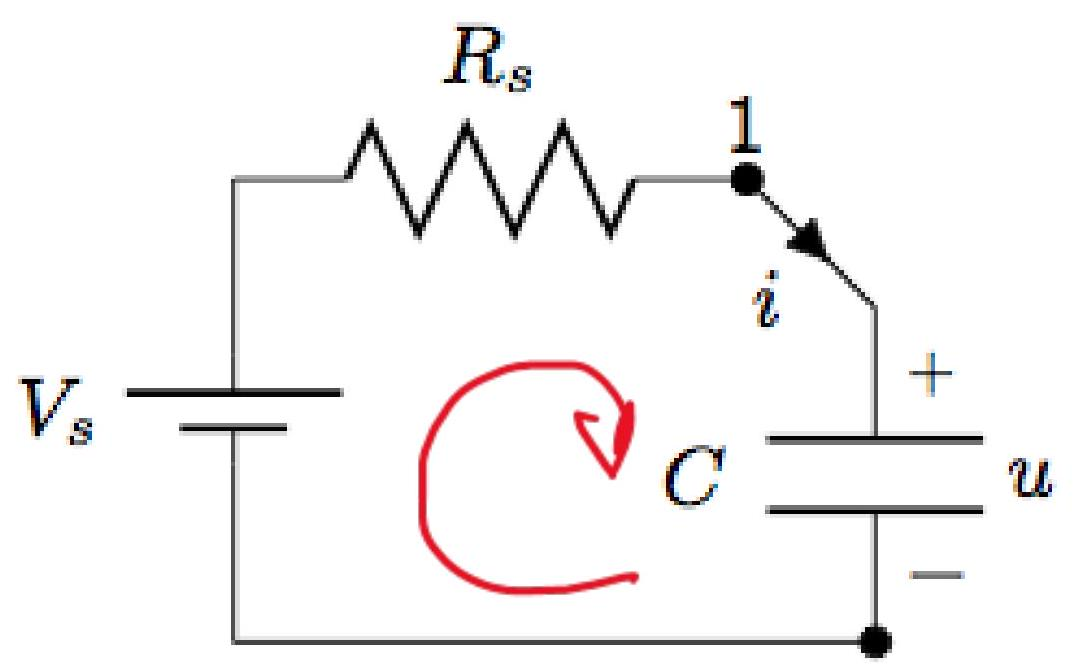
\includegraphics[width=0.6\textwidth]{images/0aae1f8e-05fc-4834-a308-b46d85861175-59_672_1079_569_265}
	\end{center}  
  \end{column}
  \begin{column}{0.45\textwidth}
	$$
	\begin{aligned}
	V_{s} & =R_{s} i+\frac{1}{C} \int_{\mathcolor{red}{-\infty}}^{t} i d t \\
	& =R_{s} i \mathcolor{red}{+u_{0}}+\frac{1}{C} \int_{\mathcolor{red}{0}}^{t} i d t
	\end{aligned}
	$$
  \end{column}
\end{columns}

\begin{columns}
	\begin{column}{0.65\textwidth}
		Le condensateur initialement chargé peut être remplacé par un condensateur initialement relaxé en série avec une source de tension constante $u_{0}$.
	\end{column}
	\begin{column}{0.2\textwidth}
	  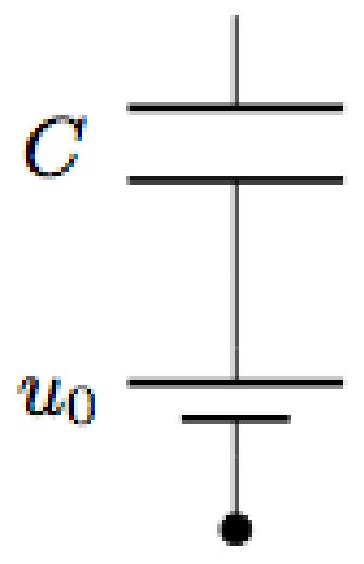
\includegraphics[width=0.4\textwidth]{images/0aae1f8e-05fc-4834-a308-b46d85861175-59_564_364_1351_596}
	\end{column}
\end{columns}

Vérifier que la tension aux bornes du condensateur est donnée par :
$$
u(t)=V_{s}\left(1-e^{-t / \tau_{s}}\right)+u_{0} e^{-t / \tau_{s}}=\text { réponse forcée }+ \text { réponse libre }
$$
\end{frame}

\section{Circuit RL}
\begin{frame}{Circuit RL}
\begin{center}
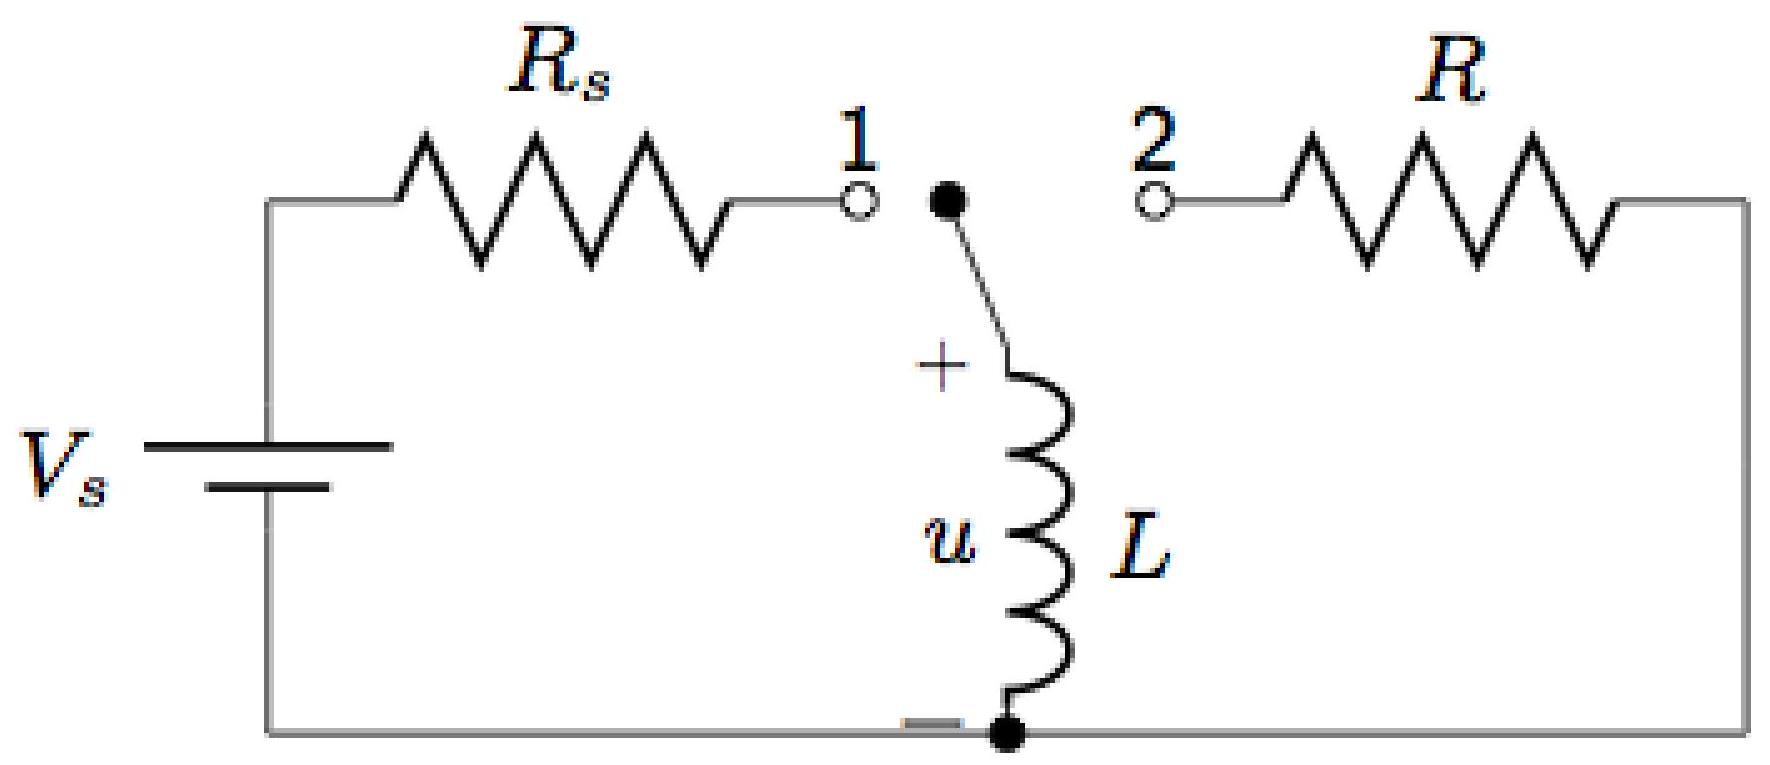
\includegraphics[width=0.4\textwidth]{images/0aae1f8e-05fc-4834-a308-b46d85861175-61_765_1770_547_1044}
\end{center}

\begin{enumerate}
  \item Interrupteur en position 1 : \textbf{réponse forcée}, établissement du courant dans l'inductance : $i_{\infty}=\frac{V_{s}}{R_{s}}$.\\
Energie magnétique emmagasinée : $w_{L}=\frac{1}{2} L i_{\infty}^{2}$.
  \item Interrupteur en position 2 : \textbf{réponse libre}, l'énergie emmagasinée dans $L$ est progressivement relachée et dissipée dans la résistance.
\end{enumerate}
\end{frame}

\begin{frame}{}

Quand $t \rightarrow \infty$\\
On suppose l'inductance initialement relaxée. En $t=0$, l'interrupteur bascule en position 1 .\\

\begin{columns}
  \begin{column}{0.45\textwidth}
	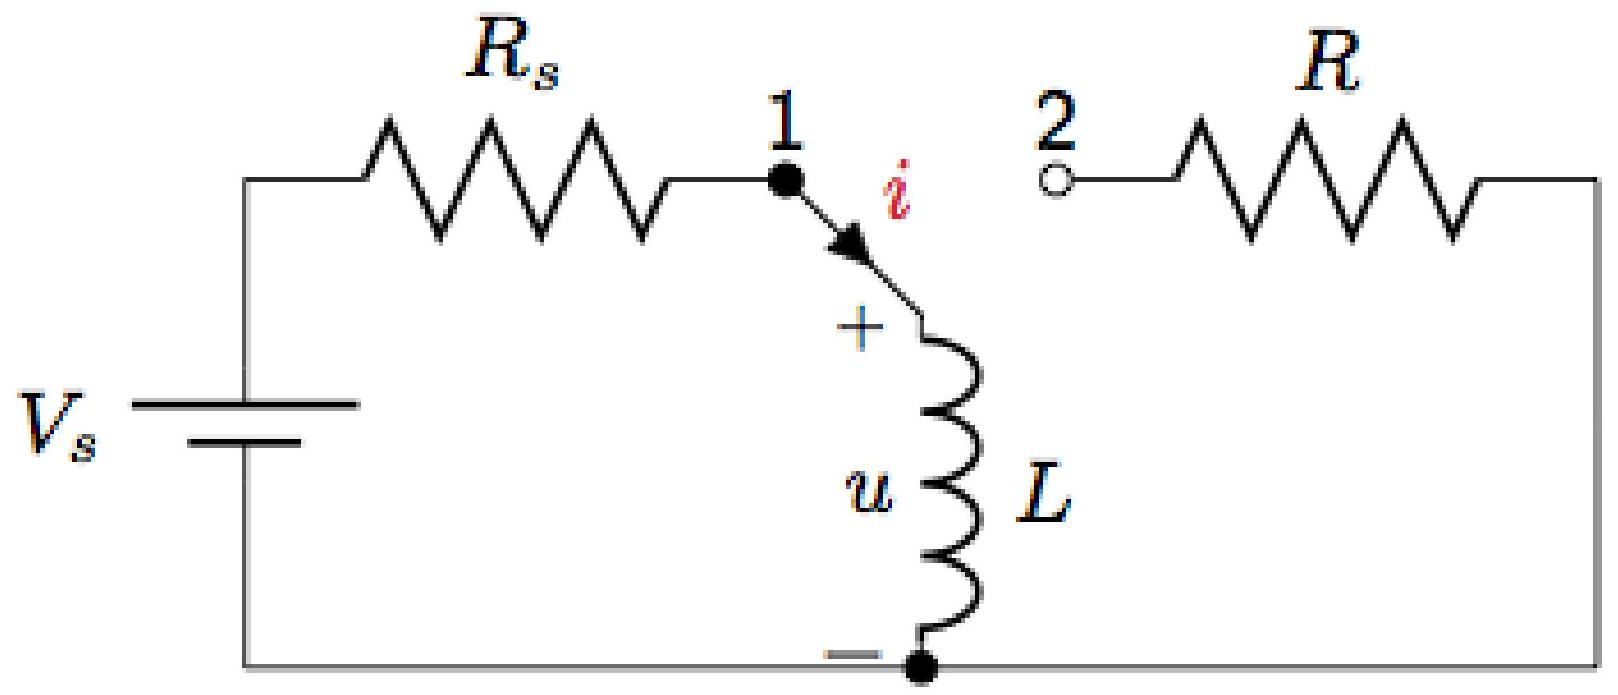
\includegraphics[width=0.8\textwidth]{images/0aae1f8e-05fc-4834-a308-b46d85861175-62_695_1618_674_356}
  \end{column}
  \begin{column}{0.45\textwidth}
	$$
	\begin{gathered}
	t<0 \quad i(t)=0 \\
	L \frac{d i}{d t}+R_{s} i=V_{s} \\
	i(t)=K e^{-t / \tau_{s}}+\frac{V_{s}}{R_{s}}
	\end{gathered}
	$$
  \end{column}
\end{columns}
Détermination de la constante K : $i(0-)=0 \rightarrow i(0+)=0$ (continuité de $i)$\\
$$
\begin{gathered}
\boxed{i(t)=\frac{V_{s}}{R_{s}}\left(1-e^{-t / \tau_{s}}\right)=i_{\infty}\left(1-e^{-t / \tau_{s}}\right) \quad t>0} \\
\lim _{t \rightarrow \infty} i(t)=\frac{V_{s}}{R_{s}}=i_{\infty}
\end{gathered}
$$

L'inductance "freine" l'établissement du courant.\\
La rapidité de cet établissement est dictée par la \alert{constante de temps} $\boxed{\tau_{s}=\frac{L}{R_{s}}}$.

\end{frame}

\begin{frame}{Remarque: quand $t \rightarrow \infty$}

\begin{columns}
  \begin{column}{0.3\textwidth}
	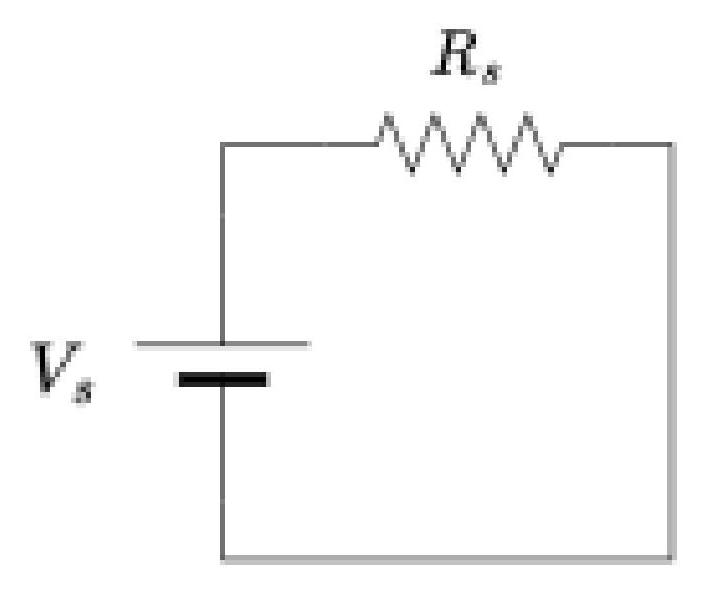
\includegraphics[width=\textwidth]{images/0aae1f8e-05fc-4834-a308-b46d85861175-62_593_708_585_3437}
  \end{column}
  \begin{column}{0.45\textwidth}
	$$
	i_{\infty}=\frac{V_{S}}{R_{S}}
	$$
  \end{column}
\end{columns}

La bobine se comporte comme un court-circuit.

\end{frame}

\begin{frame}{Evolution du courant et de la tension}
\begin{columns}
  \begin{column}{0.45\textwidth}
	$$
	\begin{aligned}
	i(t) & =i_{\infty}\left(1-e^{-t / \tau_{s}}\right) \\
	& =i_{\infty}-i_{\infty} e^{-t / \tau_{s}} \\
	& = \text{régime permanent (DC)} + \text{régime transitoire}\\
	\end{aligned}
	$$
	
	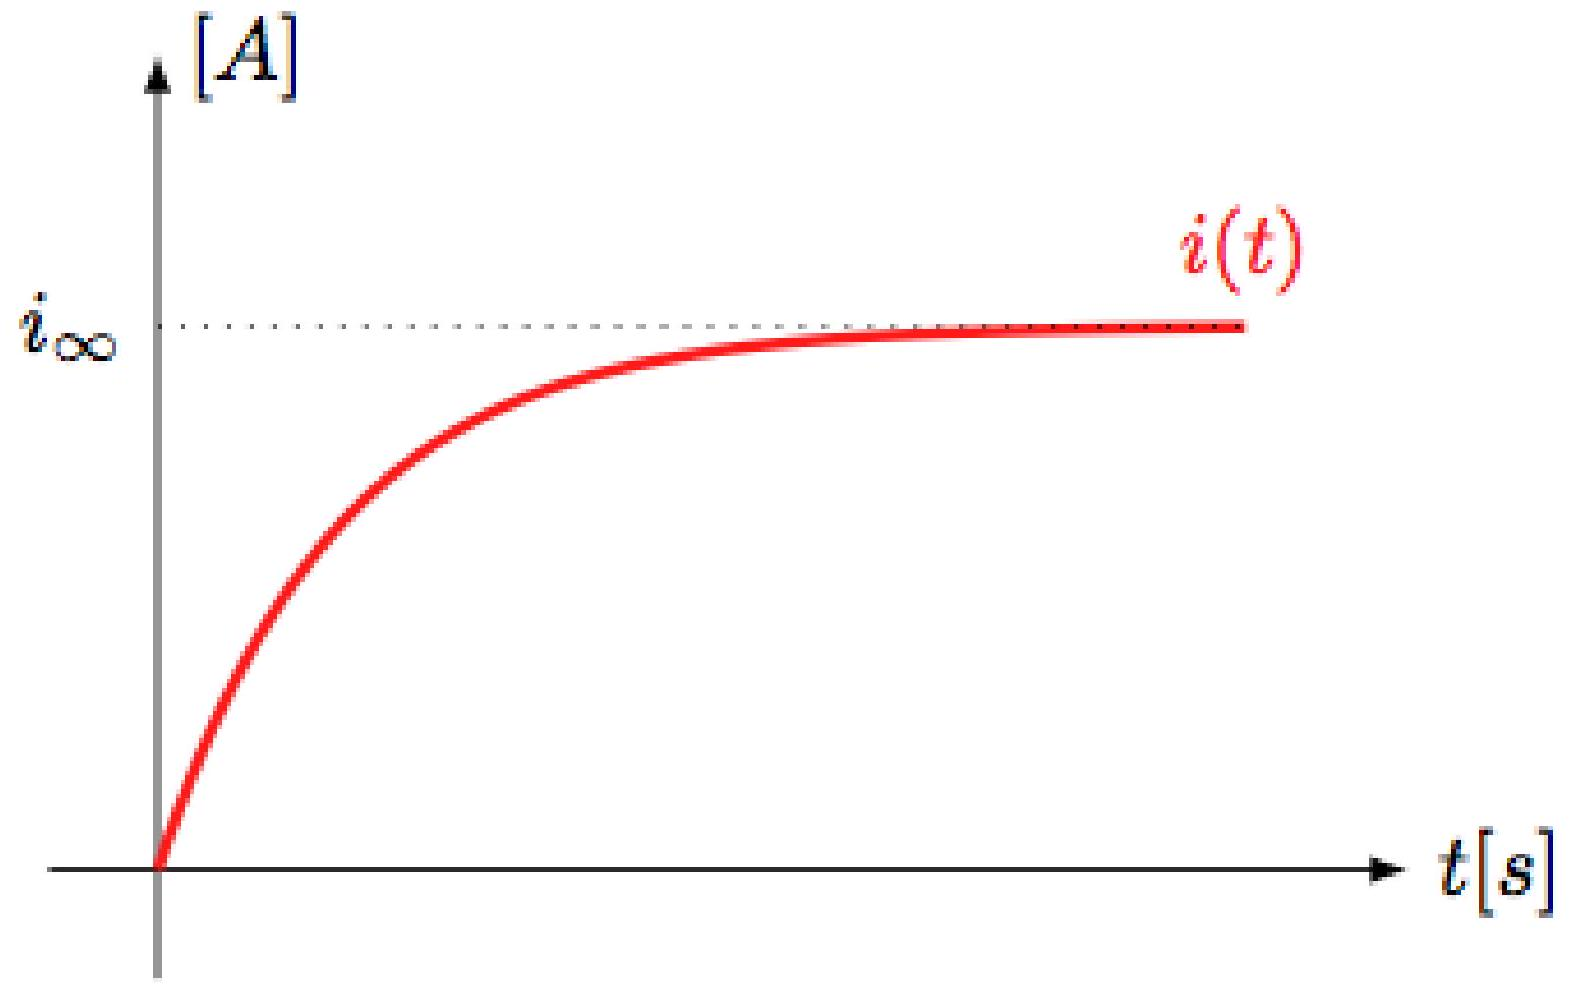
\includegraphics[width=0.8\textwidth]{images/0aae1f8e-05fc-4834-a308-b46d85861175-63_991_1569_1102_597}  
  \end{column}
  \begin{column}{0.45\textwidth}
	$$
	\begin{gathered}
	u(t)=L \frac{d i}{d t}=V_{s} e^{-t / \tau_{s}} \\
	u(0-)=0 \quad u(0+)=V_{s}
	\end{gathered}
	$$
	
	\begin{center}
	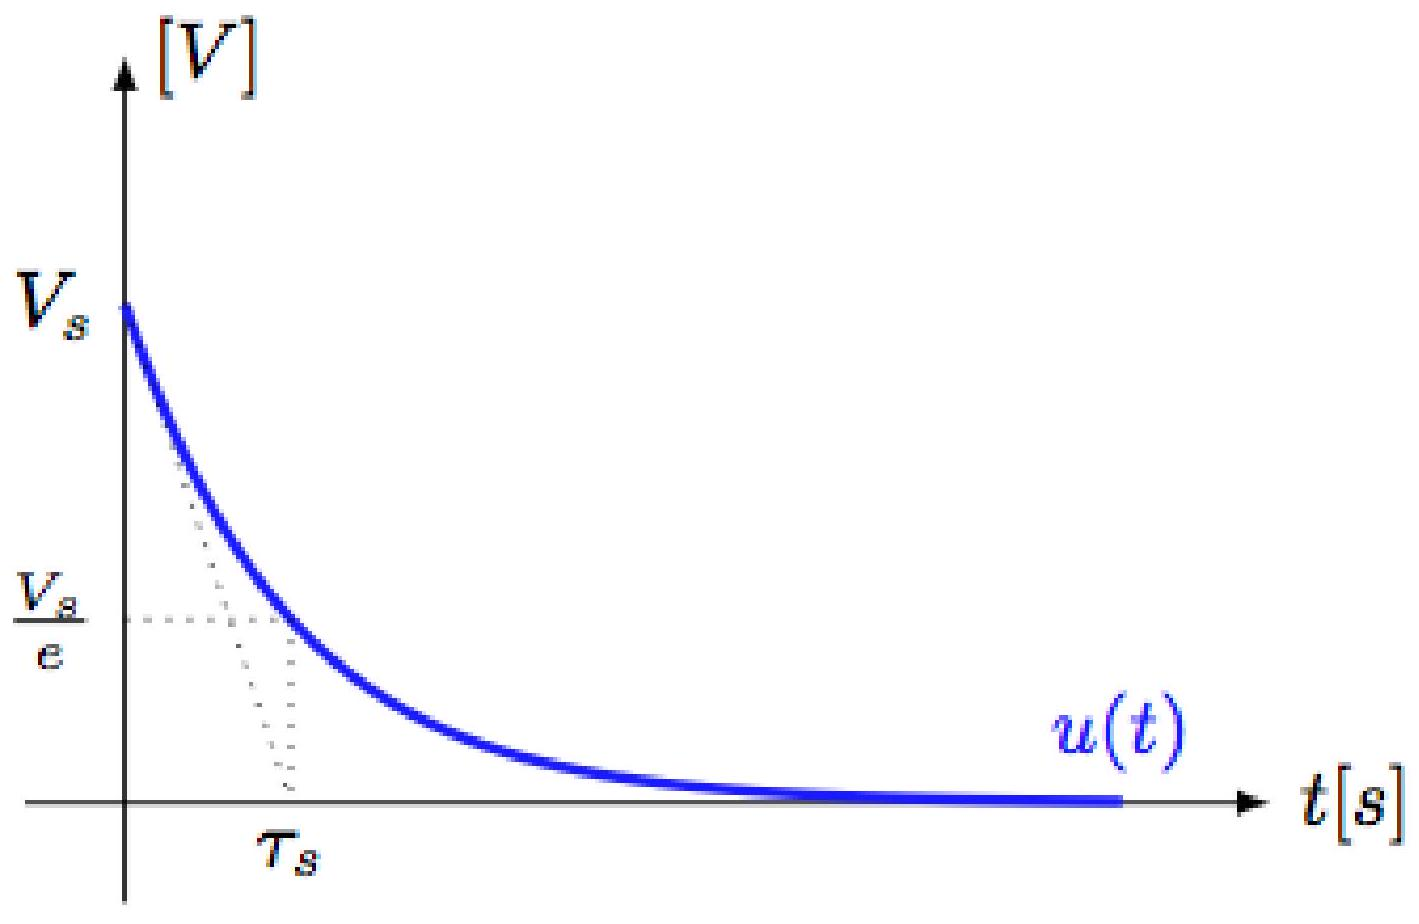
\includegraphics[width=0.8\textwidth]{images/0aae1f8e-05fc-4834-a308-b46d85861175-63_924_1419_1155_2684}
	\end{center}
  \end{column}
\end{columns}



\end{frame}

\begin{frame}[allowframebreaks]{Réponse libre}
Après un temps suffisamment long (supposé $\infty, i(t)=\frac{V_{s}}{R_{s}}=i_{\infty}$ ),\\
l'interrupteur bascule en position 2. Soit $t=0$ cet instant.

\begin{columns}
  \begin{column}{0.45\textwidth}
	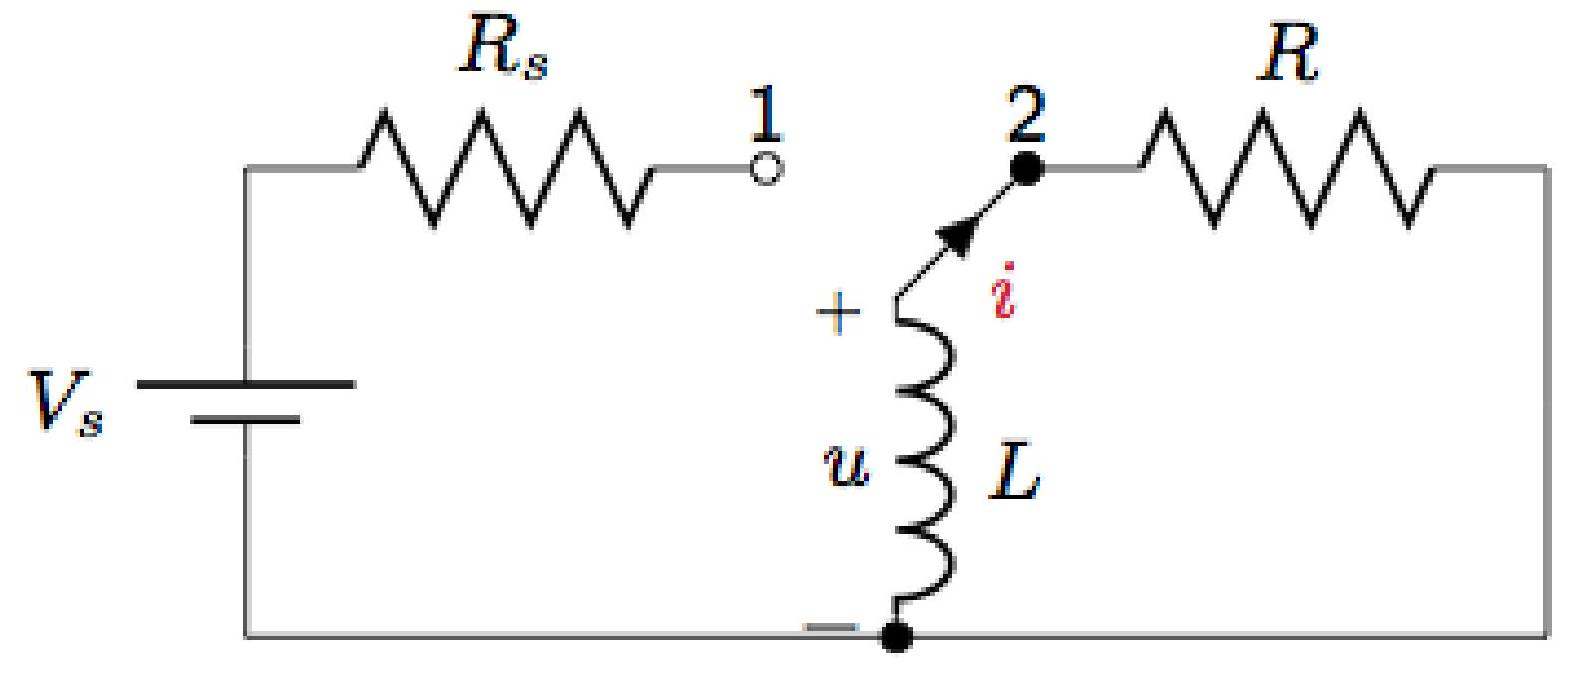
\includegraphics[width=0.9\textwidth]{images/0aae1f8e-05fc-4834-a308-b46d85861175-64_675_1579_670_330}
  \end{column}
  \begin{column}{0.45\textwidth}
	$$
	\begin{gathered}
	L \frac{d i}{d t}+R i=0 \\
	\frac{d i}{i}=-\frac{R d t}{L} \\
	i(t)=K e^{-(R / L) t}=K e^{-t /}
	\end{gathered}
	$$
  \end{column}
\end{columns}


Détermination de la constante K :
\begin{itemize}
  \item $i(0-)=i_{\infty} \rightarrow i(0+)=i_{\infty}$ (continuité de $\left.i\right)$
  \item $u(0-)=0, \quad u(0+)=R i_{\infty}$
\end{itemize}
Donc 
$$
\boxed{i(t)=i_{\infty} e^{-(R / L) t}, \quad u(t)=-R i_{\infty} e^{-(R / L) t} \quad t>0}
$$

\end{frame}

\begin{frame}{Constante de temps}
	\begin{columns}
  \begin{column}{0.4\textwidth}
	\begin{center}
	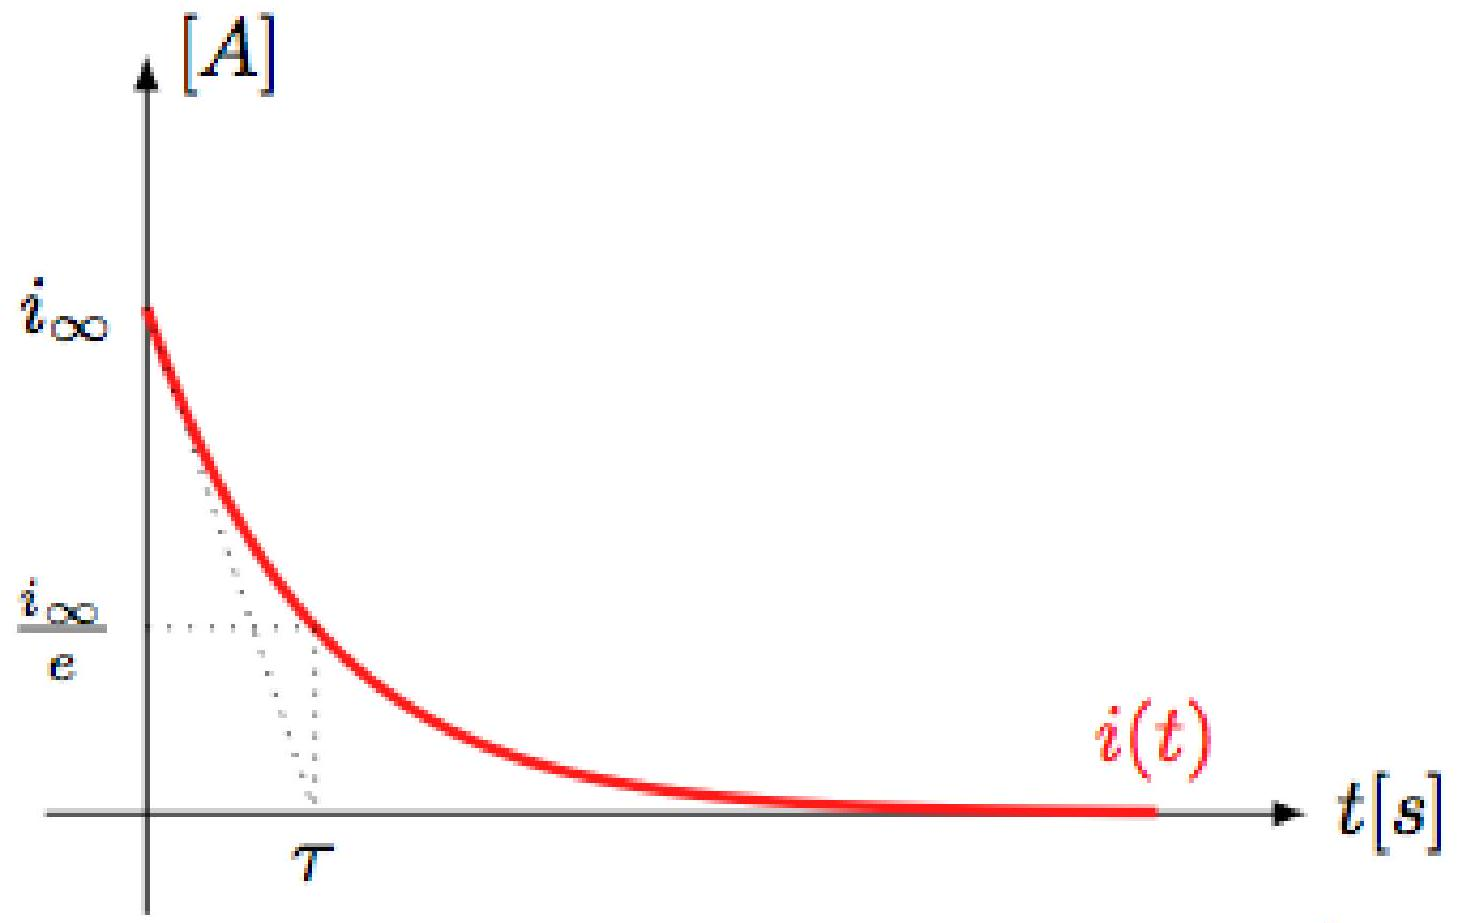
\includegraphics[width=\textwidth]{images/0aae1f8e-05fc-4834-a308-b46d85861175-65_923_1460_714_340}
	\end{center}  
  \end{column}
  \begin{column}{0.55\textwidth}
		$$
		\begin{gathered}
		\boxed{\tau=\frac{L}{R}} \\
		i(t)=i_{\infty} e^{-t / \tau} \\
		u(t)=i_{\infty} R e^{-t / \tau}
		\end{gathered}
		$$
  \end{column}
\end{columns}
		La fréquence naturelle du circuit est $-\frac{1}{\tau}=-\frac{R}{L}$

\end{frame}

\begin{frame}{Energie dissipée dans la résistance}
Puissance absorbée par la résistance :
$$
p(t)=R i^{2}(t)=R i_{\infty}^{2} e^{-2 t / \tau}>0 \quad \forall t
$$

Energie dissipée dans l'intervalle $[0, t]$ :
$$
\begin{gathered}
w(t)=\int_{0}^{t} p(x) d x=\frac{1}{2} L i_{\infty}^{2}\left(1-e^{-2 t / \tau}\right) \\
\lim _{t \rightarrow \infty} w(t)=\frac{1}{2} L i_{\infty}^{2}
\end{gathered}
$$

L'énergie initialement emmagasinée dans l'inductance est finalement entièrement dissipée dans la résistance 
à une vitesse fixée par la constante de temps $\tau$.
\end{frame}

\begin{frame}[allowframebreaks]{\large Etablissement du courant et inductance parcourue par un courant initial}
En $t=0$, l'inductance est parcourue par un courant initial $i_{0}$.\\[5mm]


\begin{columns}
  \begin{column}{0.45\textwidth}
	\begin{center}
		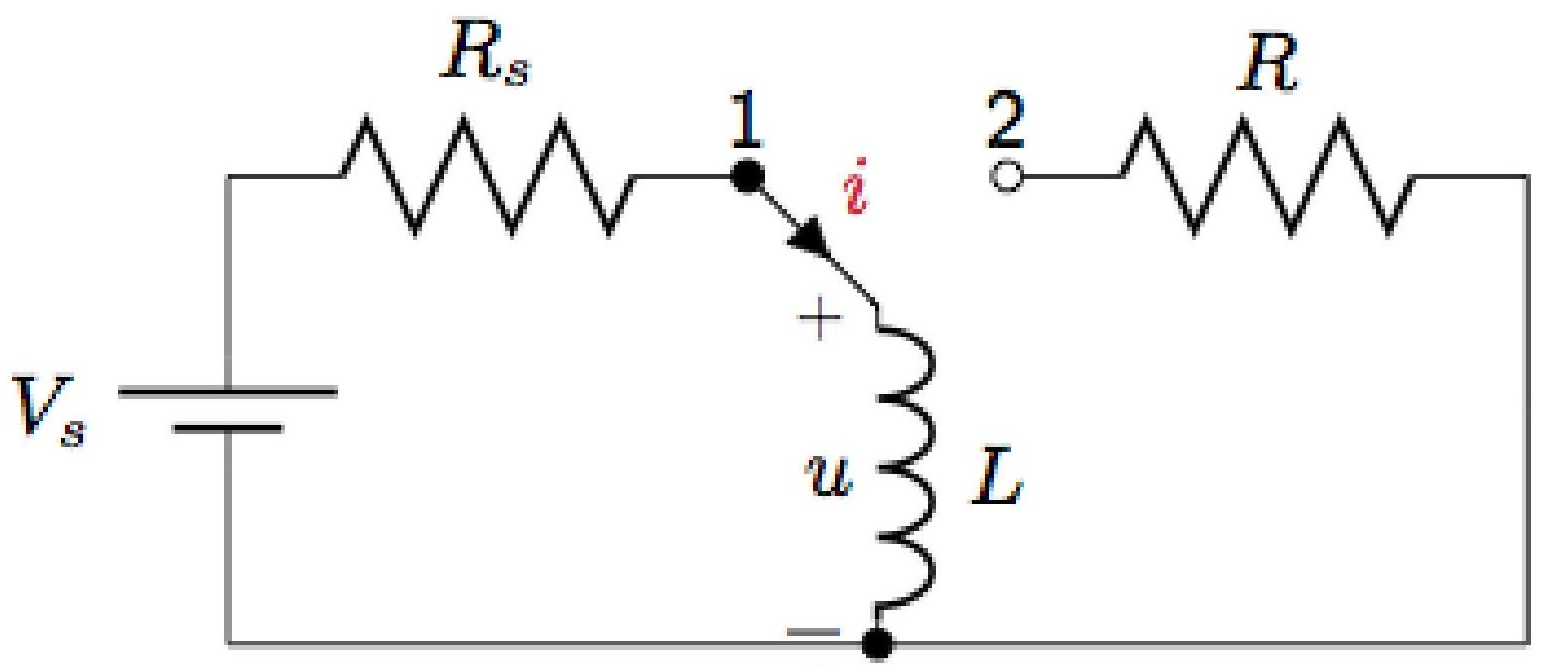
\includegraphics[width=\textwidth]{images/RL_initial.jpg}
	\end{center}
  \end{column}
  \begin{column}{0.45\textwidth}
	$$
	\begin{aligned}
	\frac{V_{s}}{R_{s}} & =\frac{u}{R_{s}}+\frac{1}{L} \int_{\mathcolor{red}{-\infty}}^{t} u d t \\
	& =\frac{u}{R_{s}}\mathcolor{red}{+i_{0}}+\frac{1}{L} \int_{\mathcolor{red}{0}}^{t} u d t
	\end{aligned}
	$$
  \end{column}
\end{columns}

\begin{columns}
  \begin{column}{0.65\textwidth}
  L'inductance initialement parcourue par un courant peut être remplacée par une inductance initialement relaxée en parallèle avec une source de courant constant $i_{0}$.
  \end{column}
  \begin{column}{0.25\textwidth}
		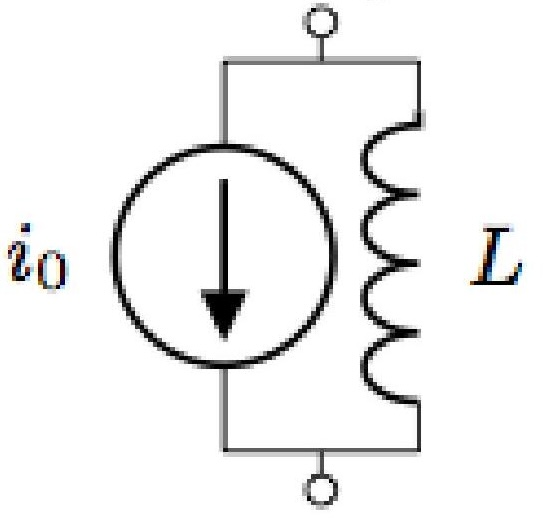
\includegraphics[width=0.6\textwidth]{images/L_initial.jpg}
  \end{column}
\end{columns}

Vérifier que le courant parcourant l'inductance est donné par :
$$
i(t)=\frac{V_{s}}{R_{s}}\left(1-e^{-t / \tau_{s}}\right)+i_{0} e^{-t / \tau_{s}}=\text { réponse forcée }+ \text { réponse libre }
$$

\end{frame}





\section{Comment résoudre un exercice en pratique ?}
\begin{frame}[allowframebreaks]{Comment résoudre un exercice en pratique}
	\begin{block} {Méthode de résolution}
		\begin{itemize}
			\item En fonction de la position d'un ou plusieurs \textbf{interrupteur}(s), de {\bf variations définies des sources} alimentant le circuit, identifier les différentes \textbf{périodes} et les circuits associés.
			\item Pour chaque période,
			\begin{enumerate}
				\item déterminer les \textbf{conditions initiales}
				\item obtenir l'\textbf{équation différentielle} de la tension (condensateur) ou du courant (inductance) en utilisant les PLK, SLK et les relations $u-i$ aux bornes des éléments
				\item résoudre cette équation différentielle
			\end{enumerate}
		\end{itemize}
	\end{block}	

\newpage
\textbf{Conseils}:
\begin{itemize}
  \item Utiliser des expressions littérales le plus loin possible, remplacer les valeurs numériques à la fin
  \item Vérifier la continuité temporelle
  \item Pour un condensateur : recherche de la tension et puis du courant par dérivation
  \item Pour une inductance : recherche du courant et puis de la tension par dérivation
  \item Vérifier les valeurs en fin et début de période par un raisonnement physique
\end{itemize}
\end{frame}


\section{Circuits du deuxième ordre -- RLC série}

\subsection{Réponse libre}
\begin{frame}[allowframebreaks]{ Réponse libre}

	Soit le circuit suivant :
	\begin{columns}
	\begin{column}{0.5\linewidth}
		\centering
		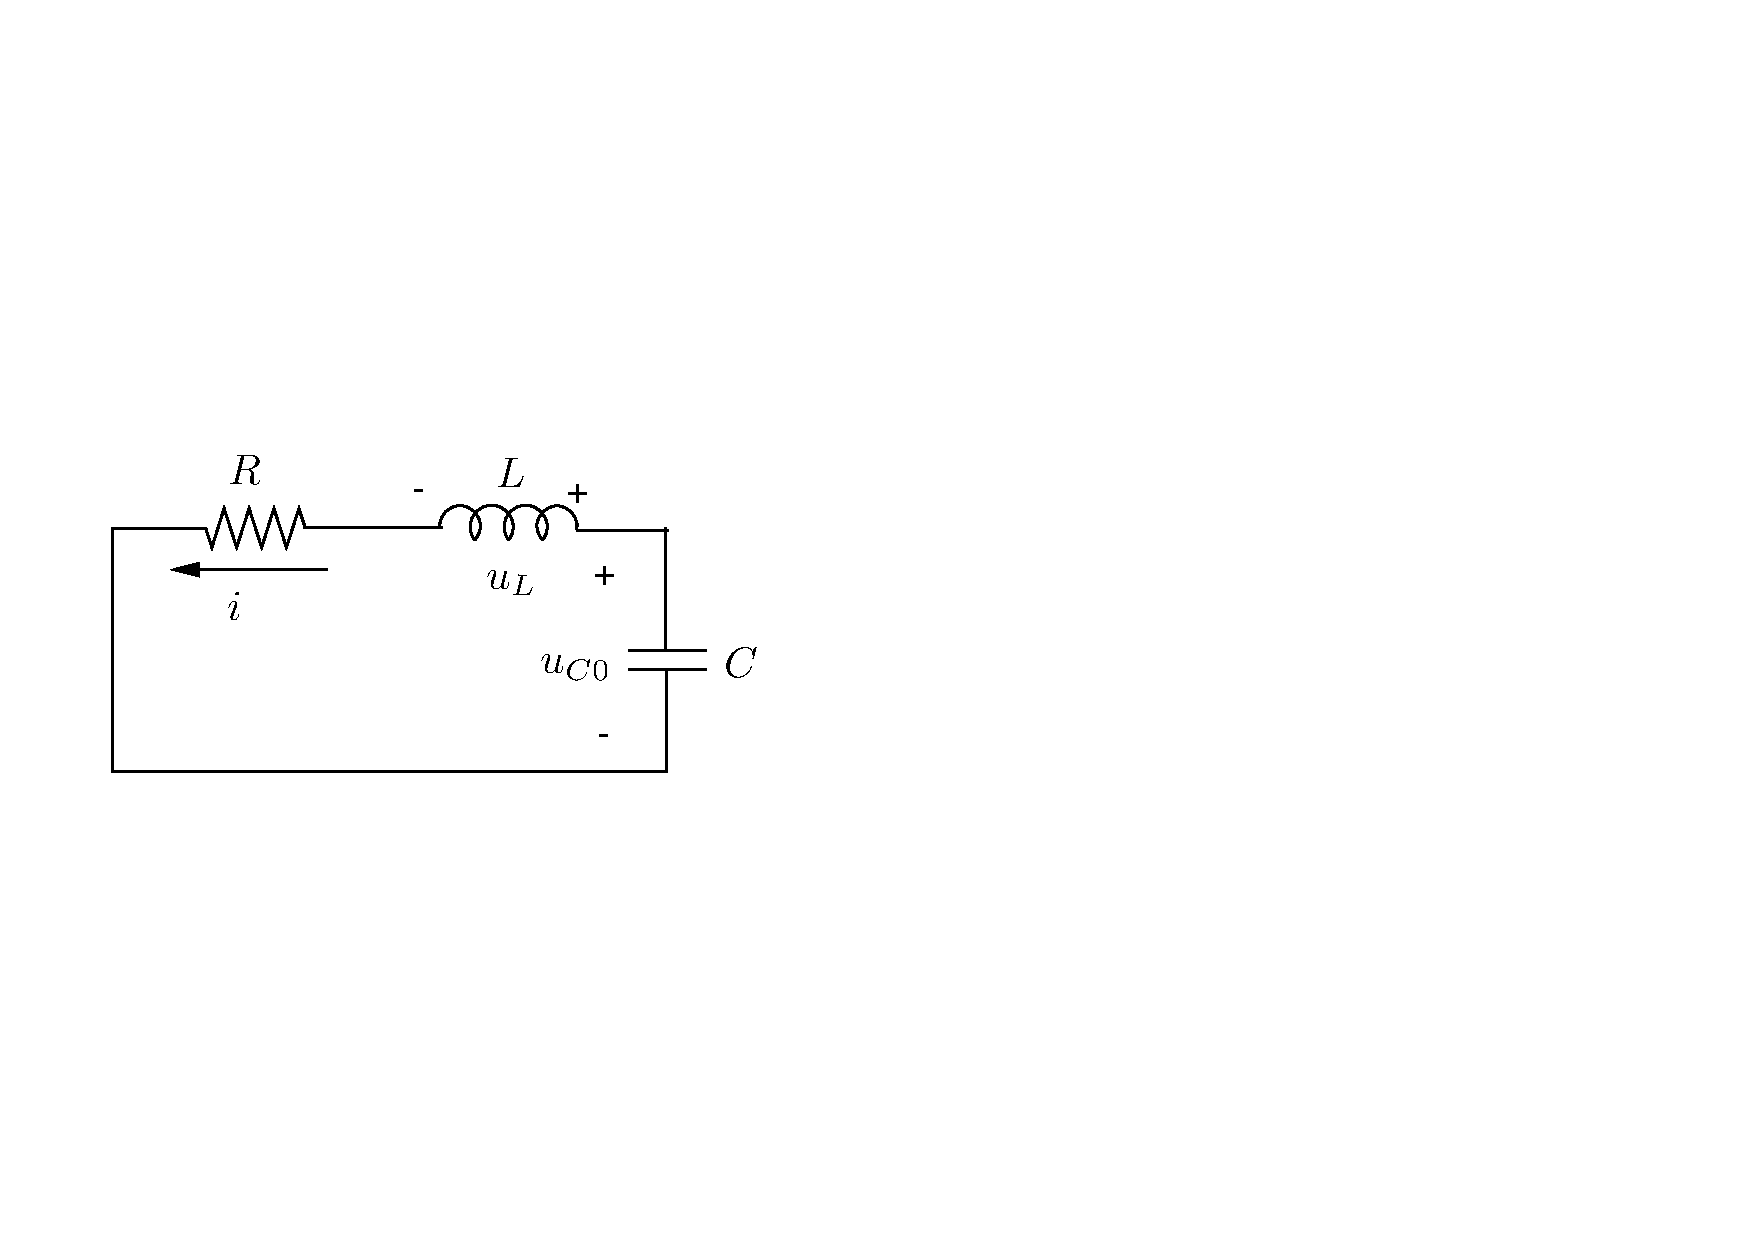
\includegraphics[width=0.7\linewidth]{images/RLC}
	\end{column}
	\begin{column}{0.45\linewidth}
	Condition initiales : 	
	\begin{enumerate}
		\item Condensateur $C$  chargé : $u_{C0}$\\
		\item Inductance relaxée : $i_0 = 0$
	\end{enumerate}	
	\end{column}
	\end{columns}
	\vfill
	Par la SLK, on a à tout instant
	\[L\frac{di}{dt}+R\, i-u_{C0}+\frac{1}{C}\int_0^t i\, dx = 0\]
	En dérivant :
	$$L\frac{d^2i}{dt^2}+R\frac{di}{dt}+\frac{1}{C} i = 0$$
	Et en divisant par $L$, on obtient 
	\begin{block} {Dynamique du circuit RLC série}
		$$\frac{d^2i}{dt^2}+\frac{R}{L}\frac{di}{dt}+\frac{1}{LC} i = 0$$
	\end{block}
\end{frame}


\begin{frame}[allowframebreaks]{Solution}
	\begin{block} {Solution générale de la forme}
		\[K_1e^{s_1 t}+K_2e^{s_2 t}\]
		où $s_1$ et $s_2$ sont les racines de l'équation caractéristique
		\[s^2 + \frac{R}{L} s + \frac{1}{LC} = 0\]
	\end{block}
\vfill
\begin{columns}
	\begin{column}{0.3\linewidth}
		Si on pose 	
		\begin{align*}
		\alpha & =  \frac{R}{2L}\\
		\omega_0 & =  \frac{1}{\sqrt{LC}}
		\end{align*}
		\end{column}
	\begin{column}{0.65\linewidth}
		alors
		\begin{align*}
		s_1 &= -\alpha + \sqrt{\alpha^2 - \omega_0^2}\\
		s_2 & =  -\alpha - \sqrt{\alpha^2 - \omega_0^2}\	
		\end{align*}
		$s_1$ et $s_2$ sont les fréquences naturelles du circuit.
	\end{column}
\end{columns}
\vfill	
	\begin{block}{3 formes de solution}
	Selon que $\alpha^2 - \omega_0^2 > 0,  \, \alpha^2 - \omega_0^2 < 0, \,\text{ ou } \alpha^2 - \omega_0^2= 0$
	\end{block}
\end{frame}

\begin{frame}{Nomenclature et intuition}
	Toutes les grandeurs $\alpha$, $\omega_0$, $s_1$ et $s_2$ sont des fréquences, mesurées en $Hz$.
	\begin{itemize}
		\item $\omega_0$ est la fréquence de résonance
		\item $\alpha$ est le coefficient d'amortissement 
		\item $s_1$ et $s_2$ sont les fréquences naturelles du circuits.
	\end{itemize}

	\vfill

	Intuition: 
	\begin{itemize}
	\item $\alpha > \omega_0 \Rightarrow $ sur-amortissement  
	\item $\alpha = \omega_0 \Rightarrow $ on est à la limite, amortissement "critique"
	\item $\alpha < \omega_0 \Rightarrow $ sous-amortissement  $\Rightarrow$ oscillations.
	\end{itemize}
	
	\vfill
	\textbf{Note:} on utilise parfois l'unité \textit{néper} ($Np$) (provient du mathématicien \textsc{John Napier})\\ pour $\alpha$, $s_1$ et $s_2$. Un néper est sans dimension. Donc, ce sont des $Np/s$ ...
\end{frame}

\begin{frame}[allowframebreaks]{Régime apériodique : $\alpha^2 - \omega_0^2 > 0 $}	
	$s_1$ et $s_2$ sont deux nombres réels {\em strictement négatifs} :
	{\small \[s_{1,2}=-\alpha \pm \sqrt{\alpha^2-\omega_0^2}= -\alpha \pm \alpha_1 < 0\]}
	Forme générale de la solution :
	{\small \[i(t)=K_1 e^{-\alpha t}e^{\alpha_1 t} + K_2 e^{-\alpha t}e^{-\alpha_1 t}\]}
	Les constantes $K_1$ et $K_2$ sont fixées par les conditions initiales:
	\begin{itemize}
		\item {\small $i(0-)=0\, \rightarrow \, i(0+)=0$ ($i$ continu dans $L$)
			\[K_1+K_2=0, \quad K_2=-K_1\]}
		\item {\small $u_R(0+)=0 \quad \text{puisque~} i(0+)=0 \rightarrow u_L(0+)=u_C(0+)=u_{C0}$
			\[u_L(0+)=\left.L\frac{di}{dt}\right|_{t=0}=\left.L(K_1s_1e^{s_1t}-K_1s_2e^{s_2t})\right|_{t=0}
			=2\alpha_1K_1L=u_{C0}\]}
	\end{itemize}
	\begin{center}
		\fbox{
			$i(t)=\frac{u_{C0}}{\alpha_1 L}\, e^{-\alpha t}\sinh (\alpha_1 t)\quad
			t\geq 0$}
	\end{center}
	
\end{frame}



\begin{frame}{Régime oscillatoire amorti : $\alpha^2 - \omega_0^2 < 0 $}

	$s_1$ et $s_2$ sont deux nombres complexes conjugués {\em à partie réelle négative}  :
	{\small \[s_{1,2}=-\alpha \pm j\sqrt{\omega_0^2-\alpha^2}= -\alpha \pm j\omega_d \]}
	Forme générale de la solution :
	{\small \[i(t)=K_1 e^{-\alpha t}e^{j\omega_d t} + K_2 e^{-\alpha t}e^{-j\omega_d t}
		= e^{-\alpha t}(K_1^{'}\cos \omega_d t + K_2^{'}\sin \omega_d t) \]}
	\[i(0+)=0 \, \rightarrow K_1^{'}=0 \qquad u_L(0+)=u_{C0}\, \rightarrow K_2^{'}=\frac{u_{C0}}{L\omega_d}\]
	\begin{center}
		\fbox{
			$i(t)=\frac{u_{C0}}{\omega_d L}\, e^{-\alpha t}\sin (\omega_d t) \quad
			t\geq 0$}
	\end{center}
\end{frame}



\begin{frame}{Régime apériodique critique : $\alpha^2 - \omega_0^2 = 0 $}	
	L'équation caractéristique possède une seule racine de multiplicité 2 :
	$$s_{1}=s_2=-\alpha < 0$$
	Forme générale de la solution (\textbf{attention}):
	$$i(t)=K_1 \mathcolor{red}{t} e^{-\alpha t}+K_2e^{-\alpha t}$$
	\[i(0+)=0 \, \rightarrow K_2=0 \qquad u_L(0+)=u_{C0}\, \rightarrow K_1=\frac{u_{C0}}{L}\]
	\begin{center}
		\fbox{
			$i(t)=\frac{u_{C0}}{L}\, t\, e^{-\alpha t} \quad t\geq  0$}
	\end{center}
\end{frame}


\subsection{Exemple}
\begin{frame}[allowframebreaks]{Exemple: Régime oscillatoire amorti}
	
	\begin{center}
		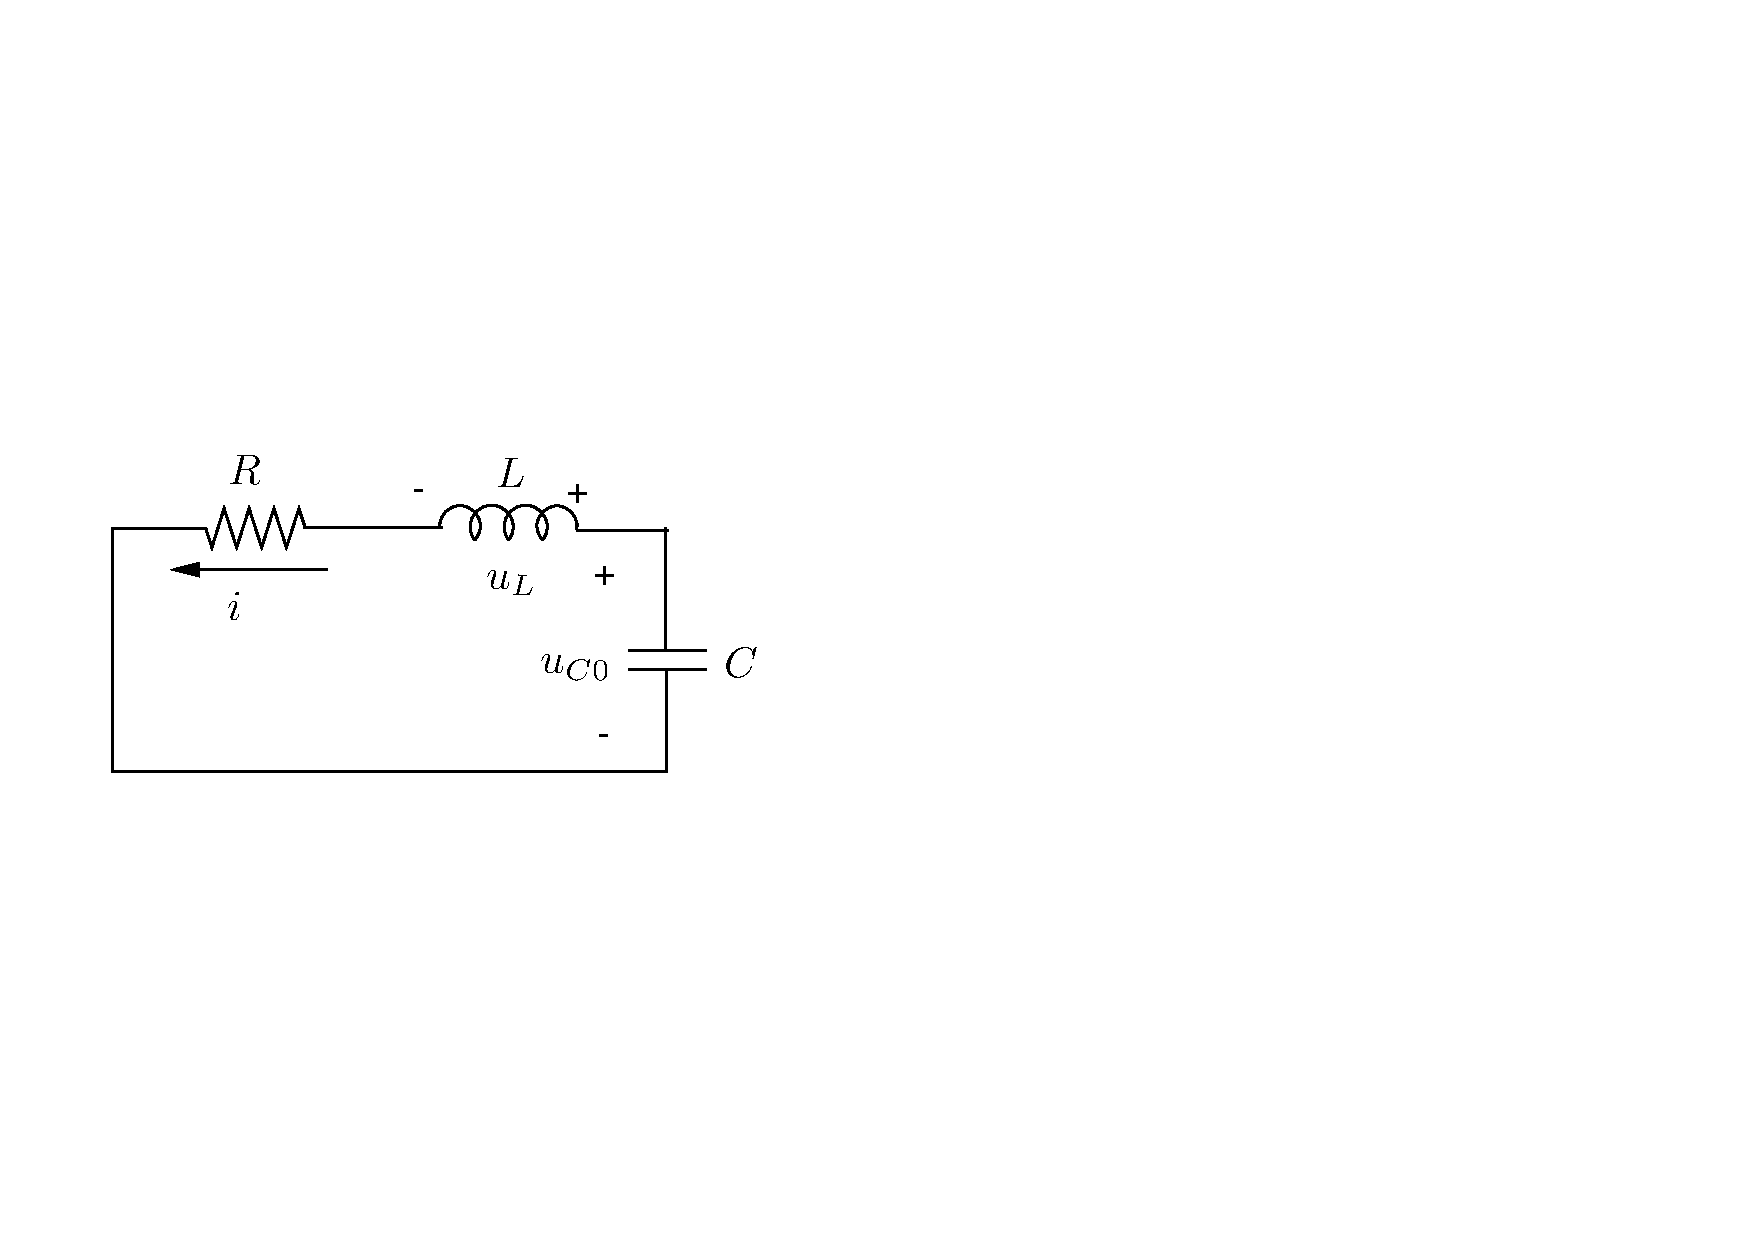
\includegraphics[width=0.4\linewidth]{images/RLC}
	\end{center}
	
	Circuit RLC série avec 
	\[\left.\begin{array}{rl}
	L=100 & \text{mH}\\
	C=0.1 & \mu\text{F}\\
	R=560 & \Omega\\
	\end{array}\right\}\rightarrow \omega_0^2=\frac{1}{LC}=10^8 \quad \alpha=\frac{R}{2L}=2800
	\]
	\[\alpha^2 < \omega_0^2 \rightarrow \quad \text{Régime oscillatoire amorti}\]
	
	Fréquence d'oscillation : $\omega_d=\sqrt{\omega_0^2-\alpha^2}=9600$ rad/s
	
	Amortissement : $\alpha=2800$ Np/s
	
	Charge initiale du condensateur : $u_{C0}=$ 100 V
	
	
	\underline{Remarque}
	
	\[\text{Si} \quad R\rightarrow 0 \text{, alors}\quad 
	\left\{
	\begin{array}{l}
	\alpha \rightarrow 0\\
	\omega_d \rightarrow \omega_0
	\end{array}\right.\]
	
	Circuit LC : régime oscillatoire non amorti, $\omega_0$ est la
	fréquence de résonance du circuit. (cfr chapitre régime sinusoïdal)

\[i(t)=\frac{u_{C0}}{L\omega_d}e^{-\alpha t}\sin\omega_d t = 0.1042e^{-2800 t}
		\sin 9600 t\quad t\geq 0\]
	
\begin{center}
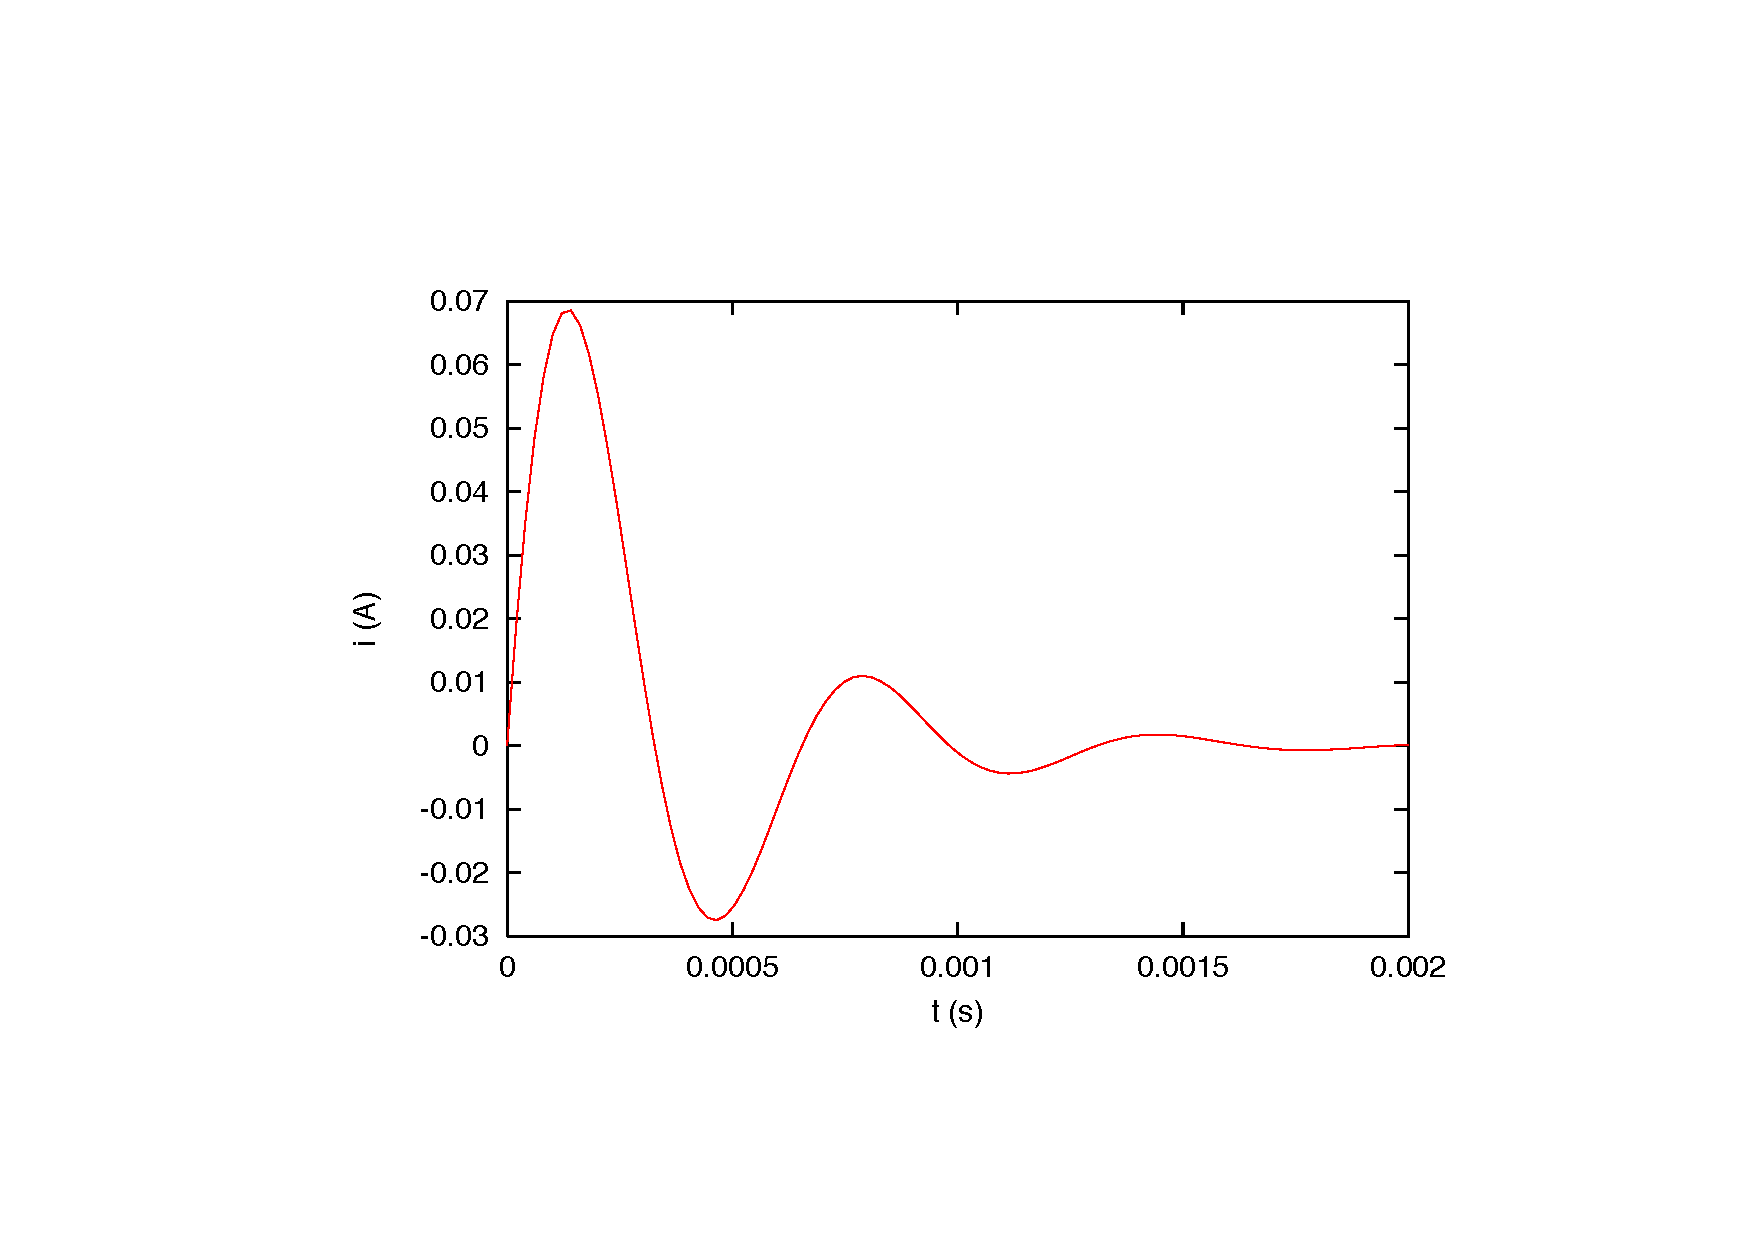
\includegraphics[width=0.6\linewidth]{images/regime_oscillatoire_amorti}
\end{center}

Calcul des tensions aux bornes des différents éléments :
	\begin{align*}
	u_R(t) &=Ri(t)\\
	u_L(t)& = L\frac{di}{dt}\\
	& = -\frac{\alpha u_{C0}}{\omega_d}e^{-\alpha t}\sin \omega_d t
	+ u_{C0}e^{-\alpha t} \cos \omega_d t\\
	& = -29.17e^{-2800 t}\sin 9600 t + 100e^{-2800 t}\cos 9600 t \quad t > 0
	\end{align*}
	On vérifie que $u_L(0+)=u_{C0}=100$
	\begin{align*}
	u_C(t)&=u_R(t)+u_L(t)\\
	& = \frac{\alpha u_{C0}}{\omega_d}e^{-\alpha t}\sin \omega_d t
	+ u_{C0}e^{-\alpha t} \cos \omega_d t\\
	& = 29.17e^{-2800 t}\sin 9600 t + 100e^{-2800 t}\cos 9600 t \quad t \geq 0
	\end{align*}
	On vérifie que $u_C(0+)=u_{C0}=100$

\begin{gather*}
		u_L(t)=-29.17e^{-2800 t}\sin 9600 t + 100e^{-2800 t}\cos 9600 t \quad t \geq 0 \quad \text{(rouge)}\\
		u_C(t)=29.17e^{-2800 t}\sin 9600 t + 100e^{-2800 t}\cos 9600 t \quad t \geq 0 \quad \text{(bleu)}
		\end{gather*}
	
\begin{center}
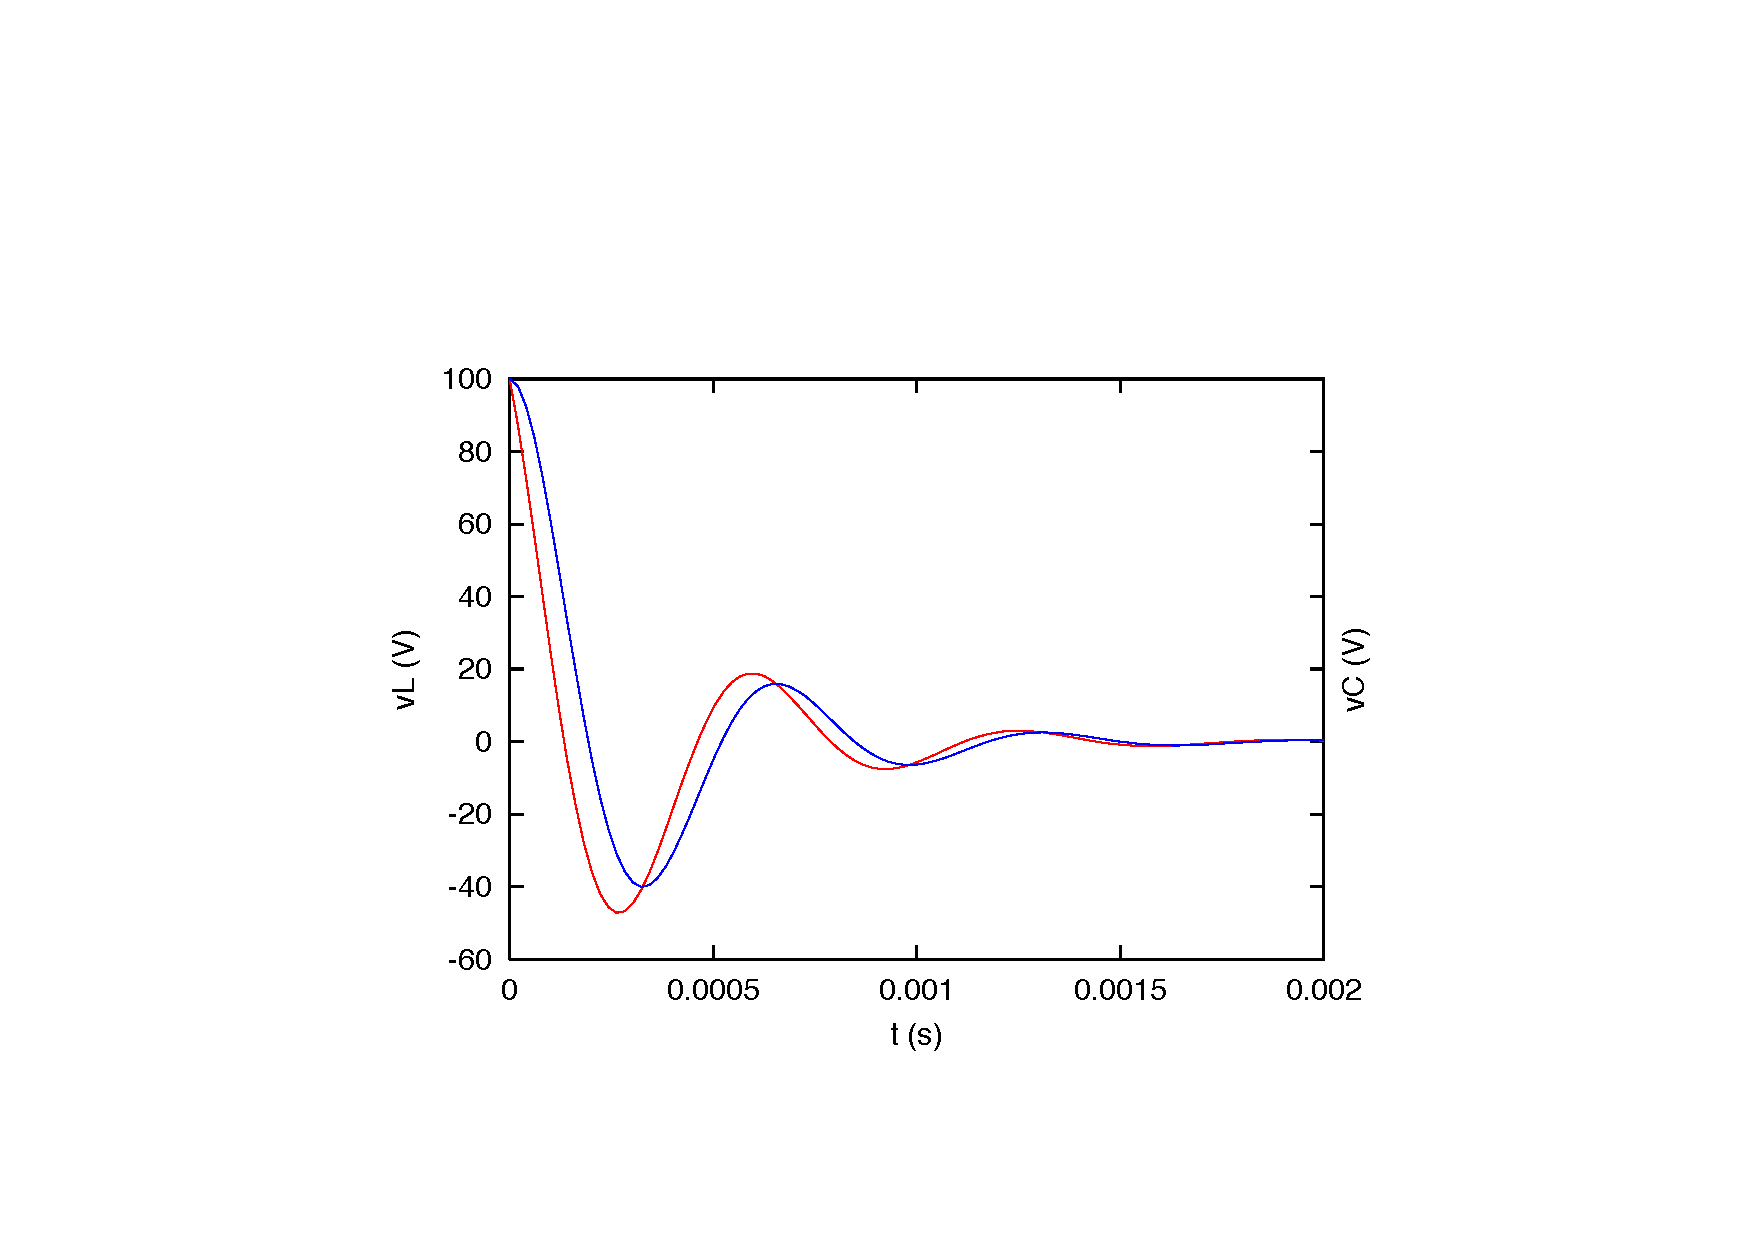
\includegraphics[width=0.6\linewidth]{images/regime_oscillatoire_amorti_u}
\end{center}
	
	Calcul des puissances consommées par les différents éléments :
	\begin{align*}
	p_R(t) &=Ri^2(t)=6.08e^{-5600 t}\sin^2 9600 t \quad > 0 \text{~~!}\\
	p_L(t) &=u_L(t)i(t) \\ &= -3.04e^{-5600 t}\sin^2 9600 t + 10.41 e^{-5600 t}\cos 9600 t \sin  9600 t\\
	p_C(t)&= -u_C(t)i(t) \\ & = -3.04e^{-5600 t}\sin^2 9600 t - 10.41 e^{-5600 t}\cos 9600 t \sin  9600 t
	\end{align*}
	
\begin{center}
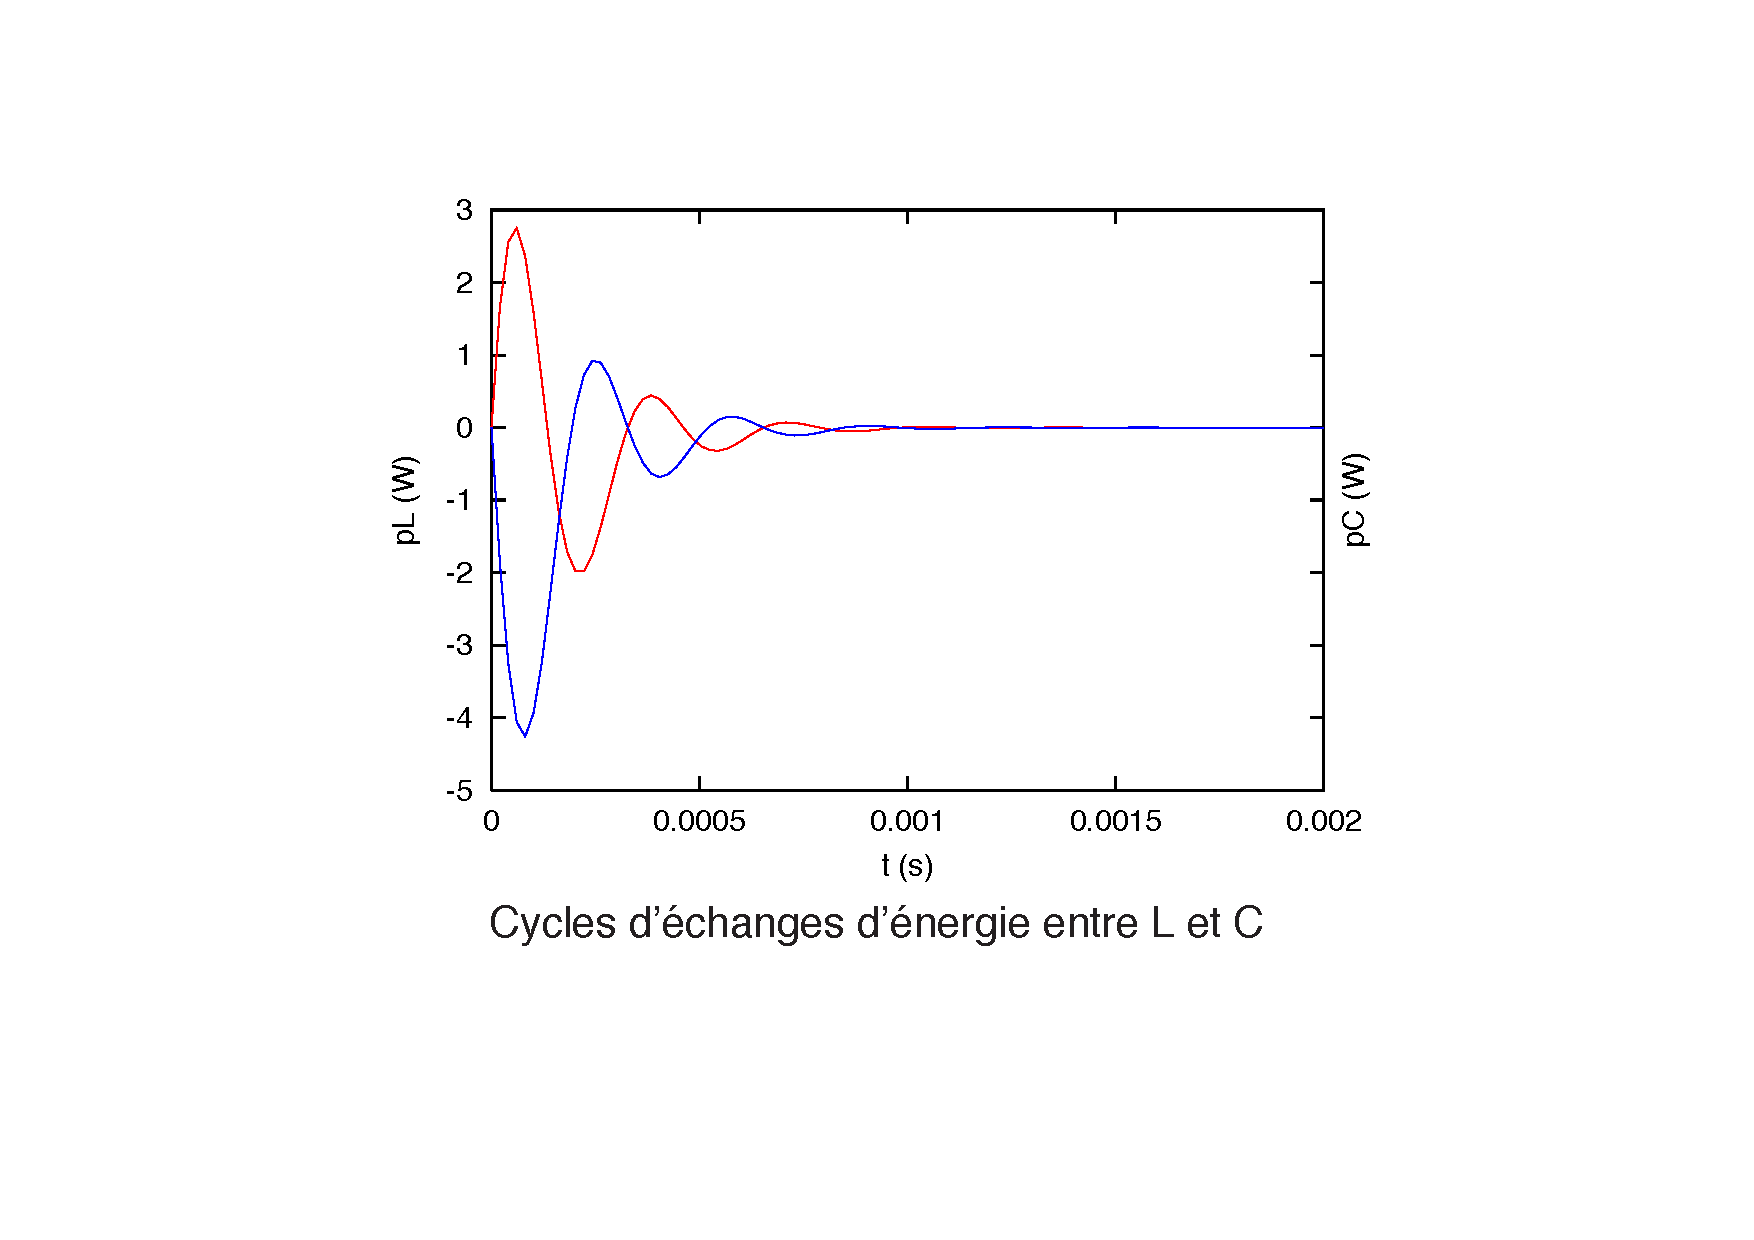
\includegraphics[width=0.7\linewidth]{images/echange_energie_L_et_C}
\end{center}
	
\end{frame}


\begin{frame}[allowframebreaks]{Régime apériodique}
		
	Circuit RLC série avec 
	\[\left.\begin{array}{rl}
	L=100 & \text{mH}\\
	C=0.1 & \mu\text{F}\\
	R=5600 & \Omega\\
	\end{array}\right\}
	\rightarrow \omega_0^2=\frac{1}{LC}=10^8 \quad \alpha=\frac{R}{2L}=28000
	\]
	\[\alpha^2 > \omega_0^2 \rightarrow \quad \text{régime apériodique}\]
	
	Deux fréquences naturelles réelles négatives :
	\begin{align*}
	s_1 &=-\alpha + \sqrt{\alpha^2-\omega^2}=-1846.6\\
	s_2 &=-\alpha - \sqrt{\alpha^2-\omega^2}=-54153.3
	\end{align*}
	
	
	Charge initiale du condensateur : $u_{C0}=$ 100 V
\begin{columns}
  \begin{column}{0.45\textwidth}
	Calcul de $i$:\\
	{\small 
		\begin{align*}
		i(t)&=\frac{u_{C0}}{2L\sqrt{\alpha^2-\omega_0^2}}e^{s_1 t}- 
		\frac{u_{C0}}{2L\sqrt{\alpha^2-\omega_0^2}}e^{s_2 t}\\
		& = 0.01912e^{-1846.6 t} - 0.01912e^{-54153.3 t}
		\end{align*}}
  \end{column}
  \begin{column}{0.45\textwidth}
	\begin{center}
	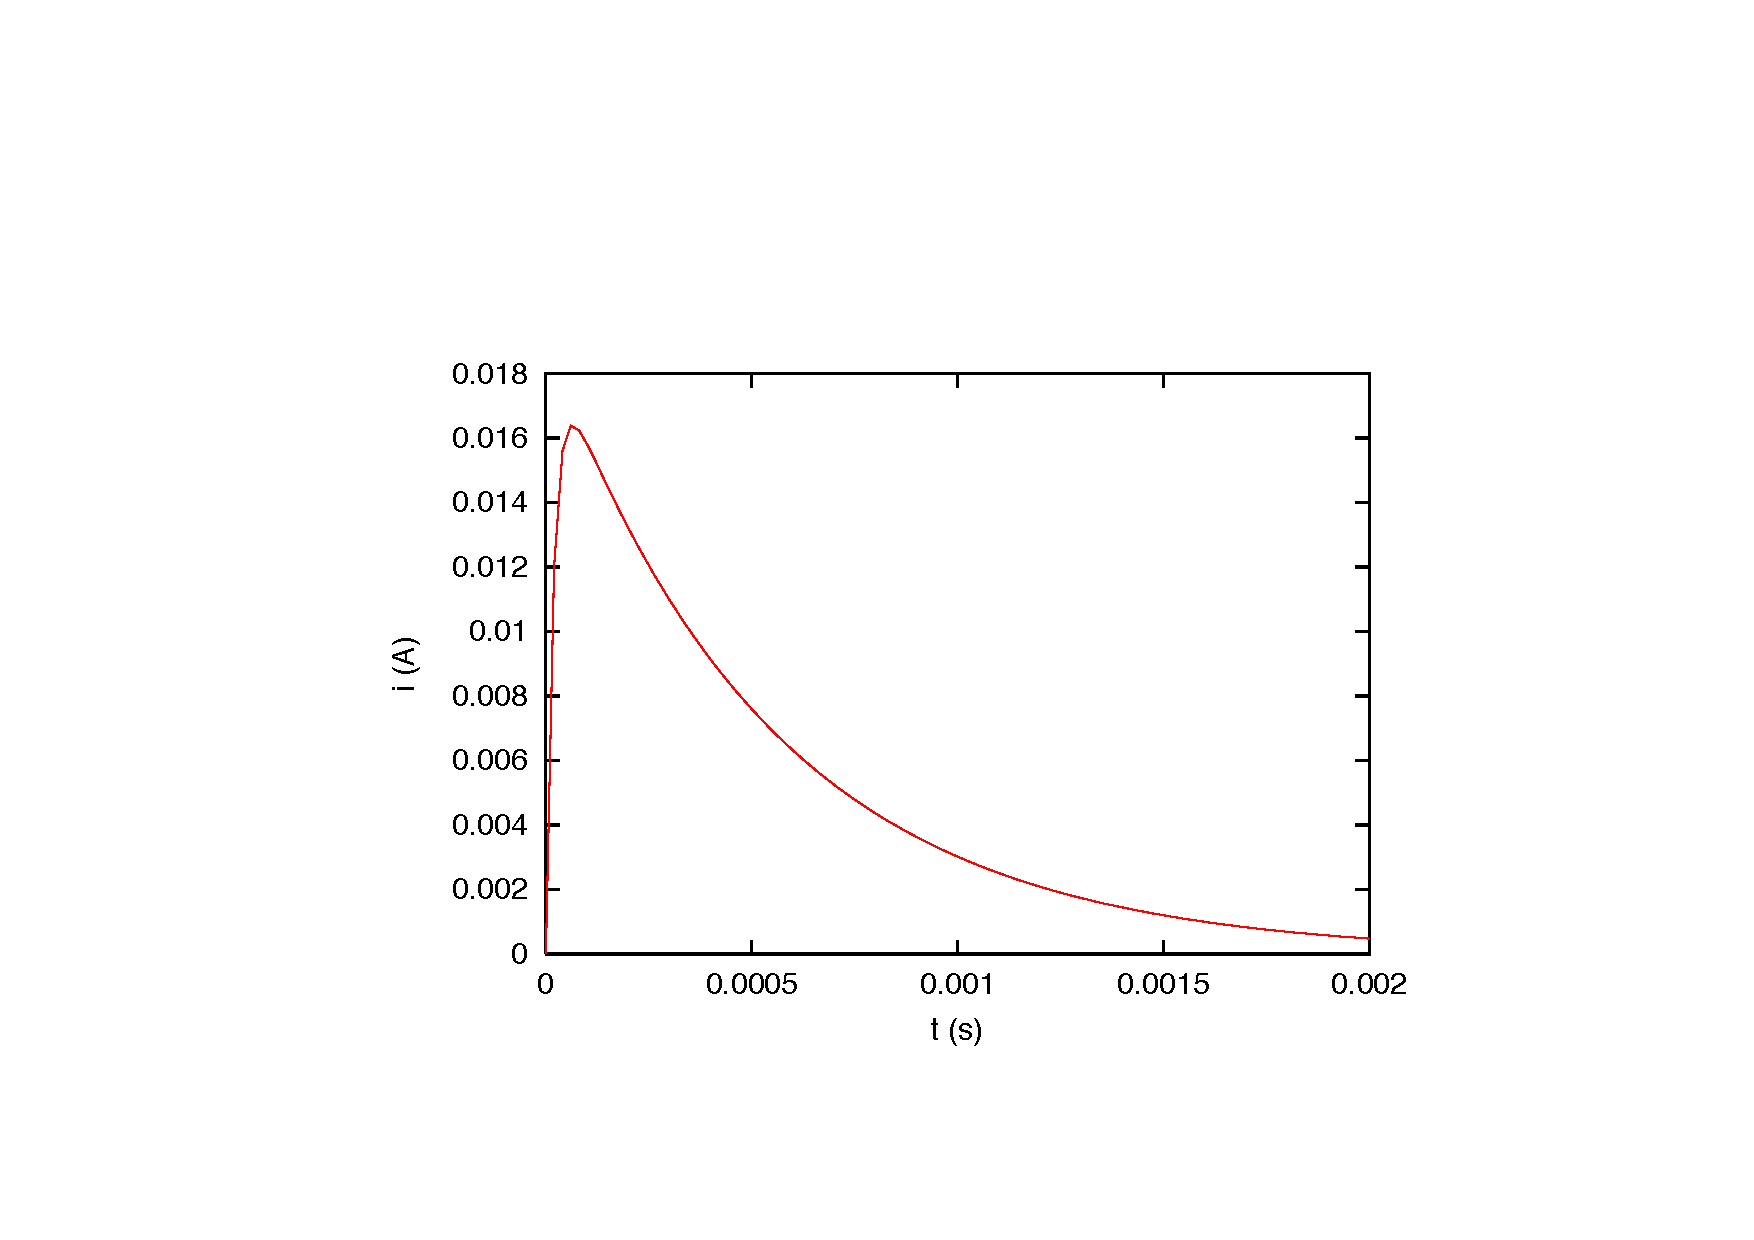
\includegraphics[width=\linewidth]{images/regime_aperiodique}
	\end{center}
  \end{column}
\end{columns}


	Calcul des tensions aux bornes des différents éléments :
	\begin{align*}
	u_R(t) &=Ri(t)\\
	u_L(t)& = L\frac{di}{dt}\\
	& =-3.53e^{-1846.6 t} +103.53e^{-54153.3 t} \quad t > 0
	\end{align*}
	On vérifie que $u_L(0+)=u_{C0}=100$
	\begin{align*}
	u_C(t)&=u_R(t)+u_L(t)\\
	& =103.53e^{-1846.6 t} -3.53e^{-54153.3 t}  \quad t \geq 0
	\end{align*}
	On vérifie que $u_C(0+)=u_{C0}=100$

	\begin{columns}
  \begin{column}{0.45\textwidth}
	Pout  $t>0$:
	{\small \begin{gather*}
		\mathcolor{red}{u_L(t)}=-3.53e^{-1846.6 t} +103.53e^{-54153.3 t}  \\
		\mathcolor{blue}{u_C(t)}= 103.53e^{-1846.6 t} -3.53e^{-54153.3 t}\\
		\end{gather*}}
  
  \end{column}
  \begin{column}{0.5\textwidth}
	\begin{center}
	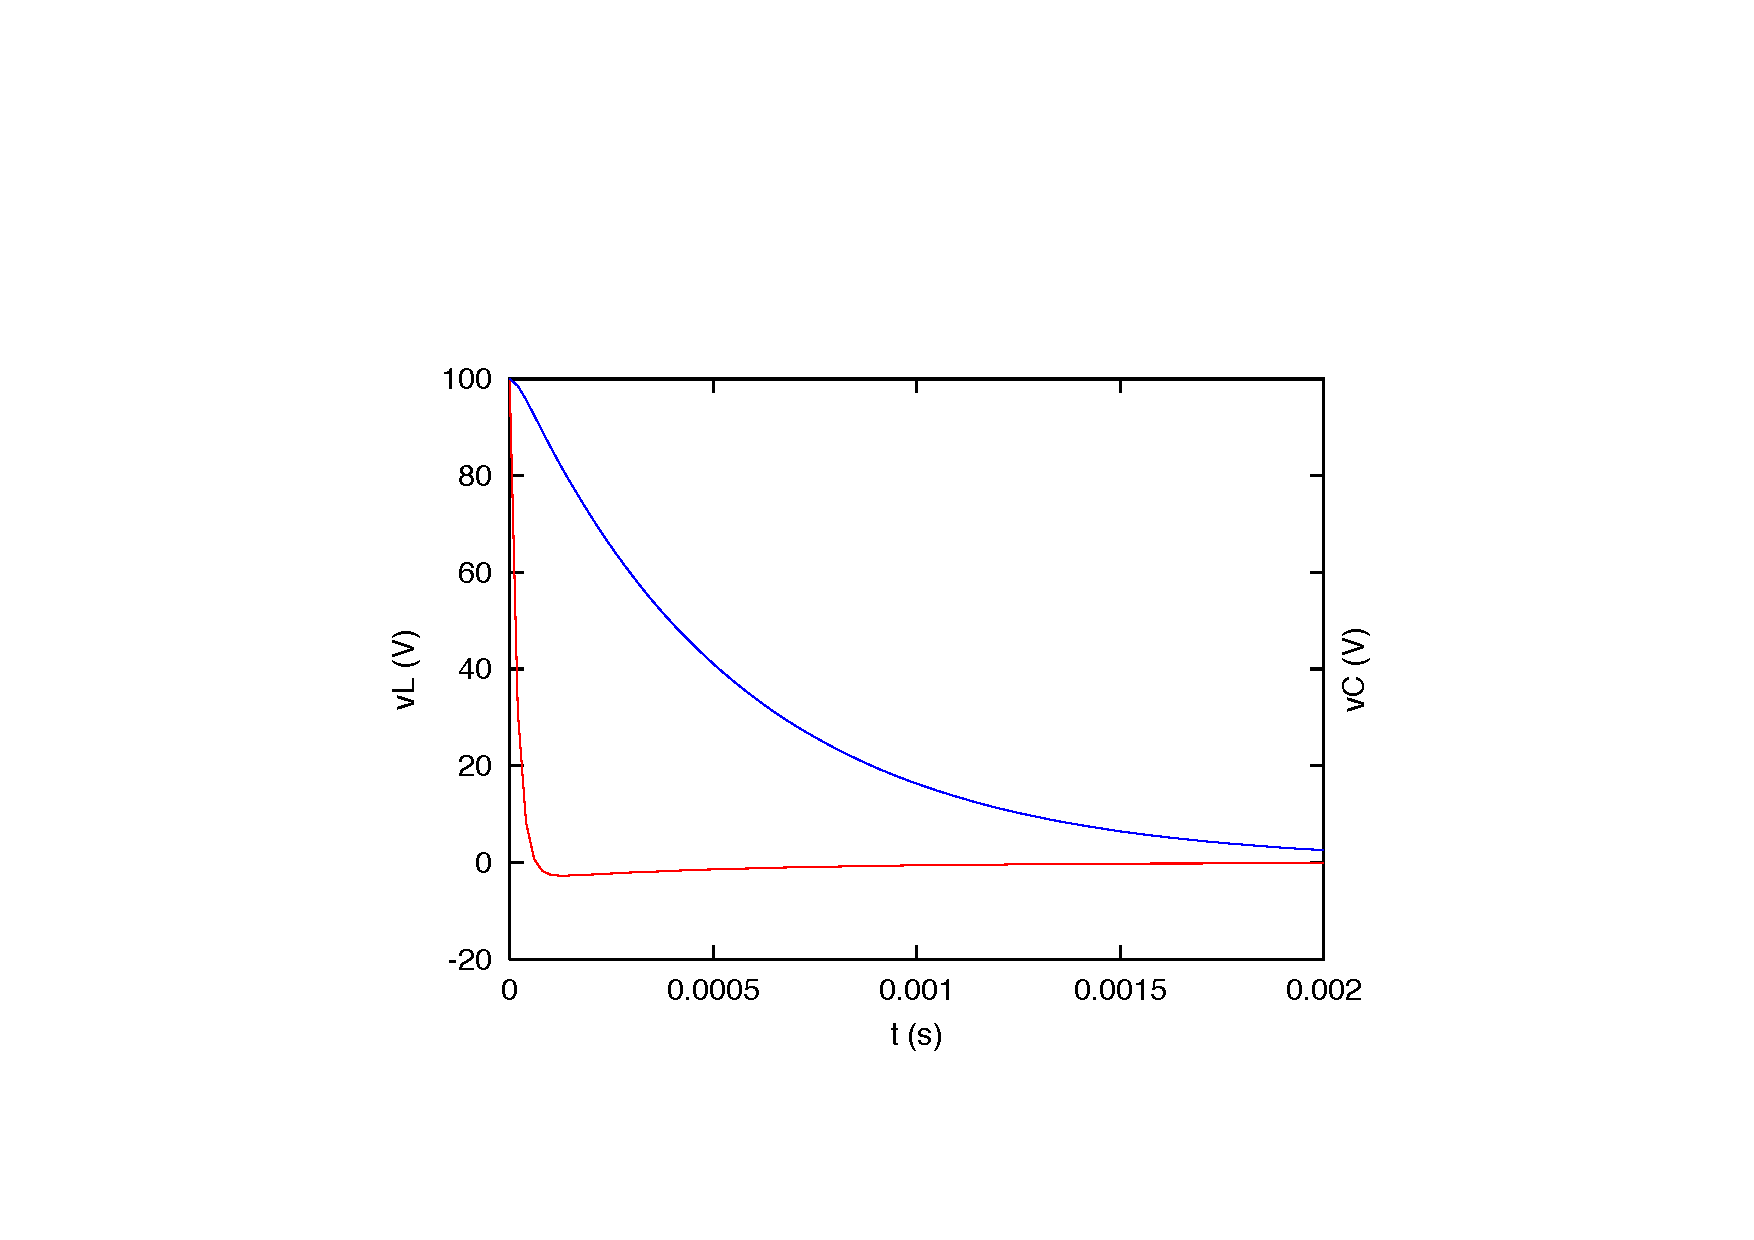
\includegraphics[width=\linewidth]{images/regime_aperiodique_u}
	\end{center}
  \end{column}
\end{columns}
	

	Calcul des puissances consommées par les différents éléments :
	\begin{align*}
	p_R(t) &=Ri^2(t) \quad > 0 \text{~~!}\\
	p_L(t) &=u_L(t)i(t) \\ &= -0.067e^{-3693.2 t}-1.98e^{-1.083\, 10^5 t}  +
	2.05e^{-56000 t} \\
	p_C(t)&= -u_C(t)i(t) \\ & =
	-1.97e^{-3693.2 t}-0.067e^{-1.083\, 10^5 t}  +
	2.05e^{-56000 t} 
	\end{align*}
	
\begin{center}
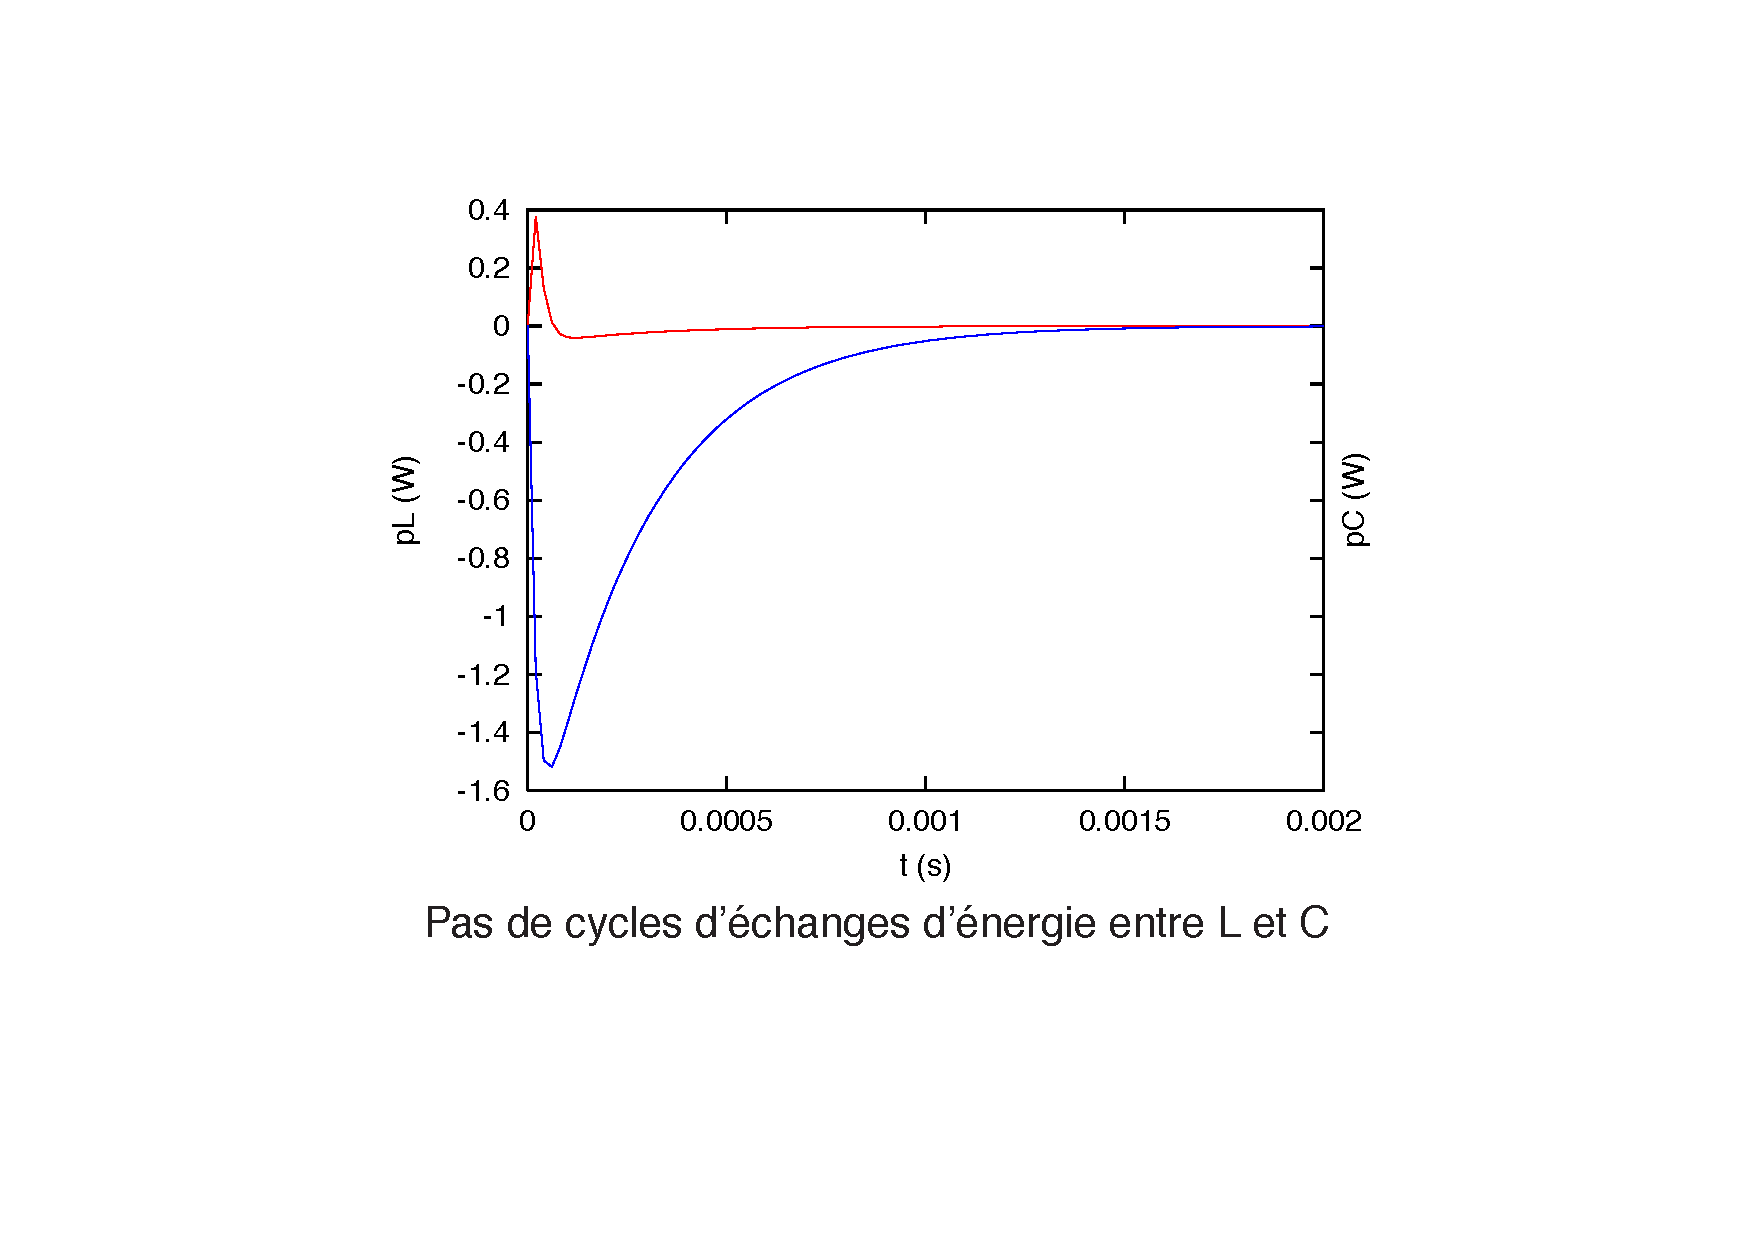
\includegraphics[width=0.6\linewidth]{images/regime_aperiodique_p}
\end{center}
	
\end{frame}



\begin{frame}[allowframebreaks]{Régime apériodique critique}	
	On obtient une racine double à l'équation caractéristique si :
	\[\frac{1}{\sqrt{LC}}=\frac{R}{2L}\]
	
	Soit pour une même valeur de $L$ et $C$, il faut :
	
	\[R=2000\,\, \Omega\]
	
	\begin{columns}
  \begin{column}{0.45\textwidth}
	\begin{align*}
	i(t) & =1000te^{-10000t}\\
	u_R(t)& =2\, 10^6te^{-10000t}\\
	u_L(t) & = 100e^{-10000t}-10^6te^{-10000t}\\
	u_C(t) & = 100e^{-10000t}+10^6te^{-10000t}
	\end{align*}
  
	{\small \[i(t)  =1000te^{-10000t}\]}
  
  \end{column}
  \begin{column}{0.45\textwidth}
	\begin{center}
	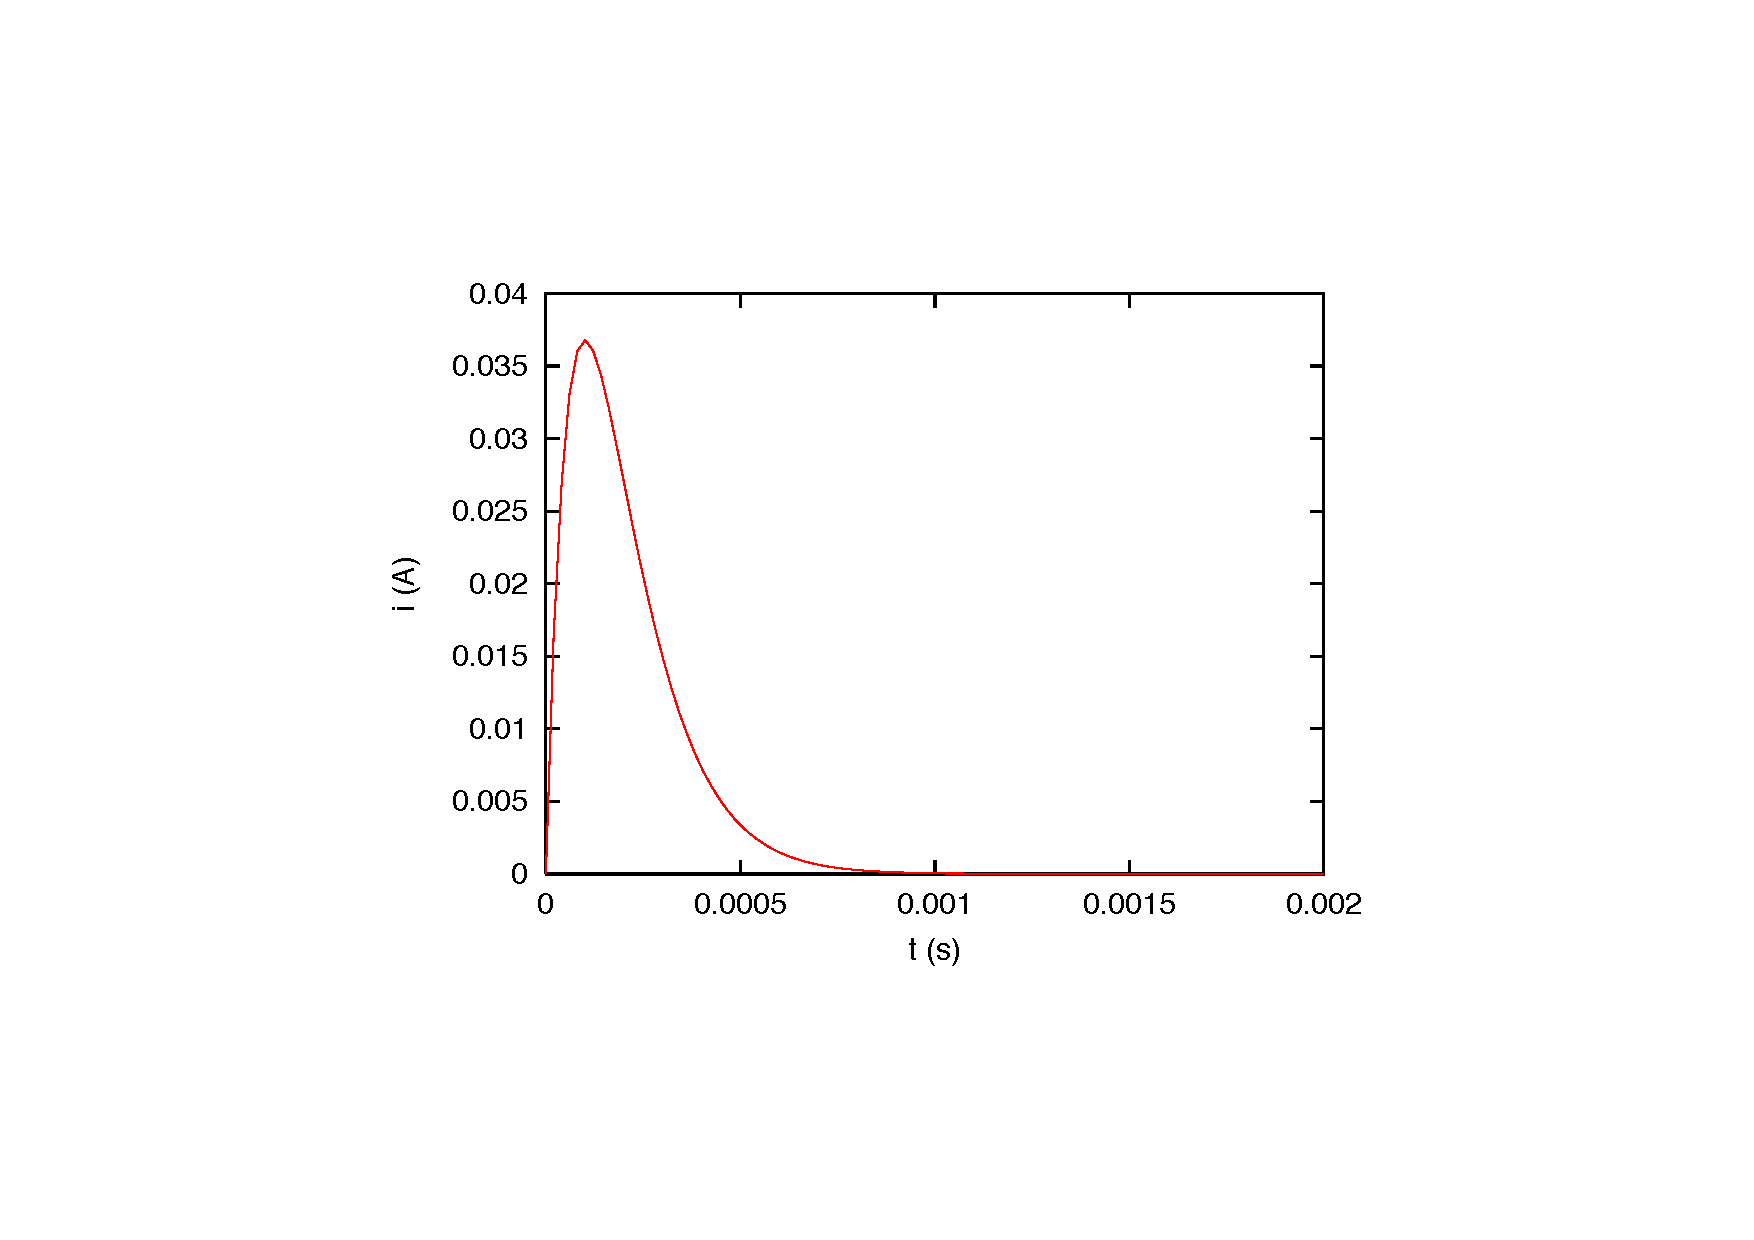
\includegraphics[width=\linewidth]{images/regime_aperiodique_critique}
	\end{center}
  \end{column}
\end{columns}
\end{frame}


%\subsection{Résolution numérique}
%
%\begin{frame}{Résolution numérique}
%	Reprenons l'équation différentielle qui régit l'exemple précédent :
%	$$\frac{d^2i}{dt^2}+\frac{R}{L}\frac{di}{dt}+\frac{1}{LC} i = 0$$
%	avec $u_{C0}=$ 100 V.
%	
%	\vfill
%	
%	\begin{block}{Question :}
%	Comment résoudre cette équation "numériquement" ?
%	\end{block}
%
%	\vfill
%
%	Utilisons une méthode de résolution numérique (d'intégration) d'équation différentielle ordinaire en Python.
%\end{frame}


%\begin{frame}{Résolution numérique - reformulation}
%	
%Les méthodes de résolution numérique nécessitent généralement de reformuler les équations de degré supérieur à 1 en un système d'équations du premier degré du type
%$$\frac{d\mathbf{x}}{dt} = A\mathbf{x} + b$$
%où $\mathbf{x}$ est un vecteur de dimension $n$ tel que $x_i = \frac{dx_{i-1}}{dt}$, pour $i \in \{ 2, ..., n\}$. Le nombre $n$ est le degré de l'équation différentielle de départ.
%Dans notre cas $n=2$, $x_1 = i$, et $x_2 = \frac{di}{dt}$.
%On a donc le système
%\begin{align*}
%\frac{dx_1}{dt} &= x_2 \\
%\frac{dx_2}{dt} &= -\frac{1}{LC} x_1 - \frac{R}{L} x_2\\
%\end{align*}
%\end{frame}
%
%\begin{frame}[containsverbatim]{Résolution numérique - code}
%Voir \url{https://github.com/bcornelusse/ELEC0053-circuits-electriques/blob/master/RT/RLC.py}
%\end{frame}

%\begin{frame}[containsverbatim]{Résolution numérique - code - paramètres}
%\begin{python}
%# -*- coding: utf-8 -*-
%
%# Example numerical solution of RLC circuit, 
%# for the free response case.
%
%from scipy import integrate  # for ODE solution
%from pylab import *  # for plotting commands
%
%# Parameters
%R_0 = 560.  # Ohm
%L = 0.1  # 100 mH
%C = 0.1e-6  # 0.1 microF
%u_c0 = 100  # V, initial voltage accross C
%\end{python}
%\end{frame}
%
%
%\begin{frame}[containsverbatim]{Résolution numérique - code - dynamique et conditions initiales}
%	\begin{python}
%def rlc(A, t):
%	"""The function that encodes the dynamics of 
%	the RLC circuit."""
%	
%	# x_1 represents i, x_2 represents di/dt
%	x_1, x_2 = A  
%	rhs = array([x_2, (-1/(L*C)*x_1 - R/L*x_2)])
%	return rhs
%
%# Pay attention to the initial conditions
%initial_conditions = [0, u_c0/L]  
%\end{python}
%\end{frame}
%
%\begin{frame}[containsverbatim]{Résolution numérique - code - résolution pour $i$, préparation }
%\begin{python}
%# Simulation period: time spans around 2 ms, 
%# divided in 1000 intervals
%time = linspace(0.0, 2e-3, 1001)
%
%# Create a figure environment for plotting.
%figure()
%
%# List of resistor values we are going to simulate 
%R_list = [R_0, 2000, 10*R_0]
%legend_names = ["$R=%.0f \Omega$" % r for r in R_list] # for plotting
%\end{python}
%\end{frame}
%
%\begin{frame}[containsverbatim]{Résolution numérique - code - résolution pour $i$ }
%\begin{python}
%for r in R_list:
%	R = r  # Global variable, changes value used in rlc()
%	# This is where the solution takes place.
%	i, di = integrate.odeint(rlc, initial_conditions, time).T
%	# i now contains the evolution of the current
%	# di now contains the evolution of the time derivative 
%	# of the current
%	plot(1000*time, i)
%
%# Plot formating
%legend(legend_names)
%xlabel('$t$ [ms]')
%ylabel('$i(t)$ [A]')
%show()
%\end{python}
%\end{frame}
%
%\begin{frame}{Résolution numérique - résultat}
%\begin{center}
%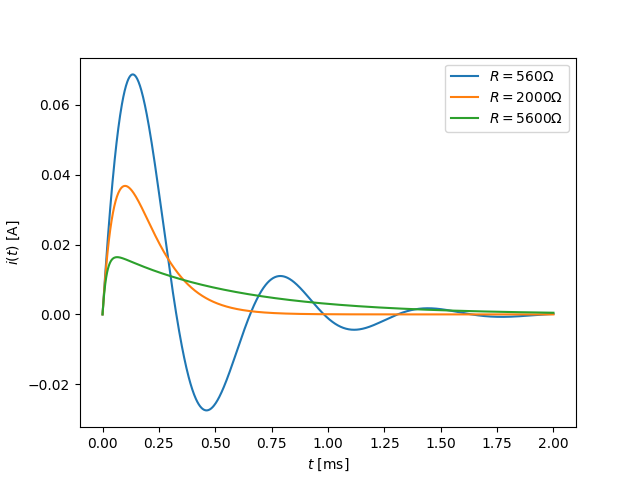
\includegraphics[width=0.6\linewidth]{exemple_numerique_i}
%\end{center}
%\end{frame}
%
%\begin{frame}{Résolution numérique - résultat}
%\begin{center}
%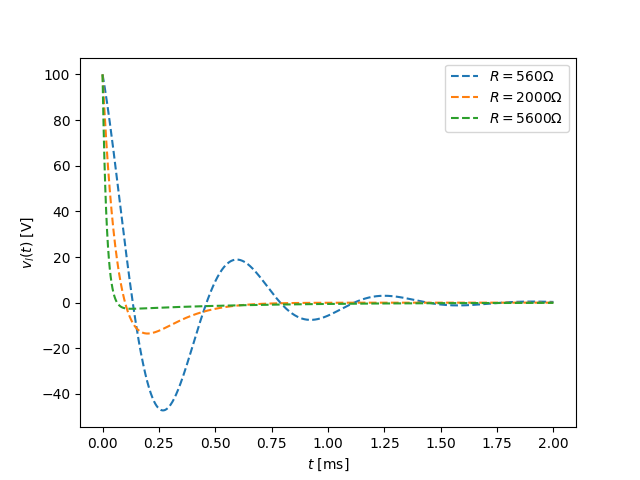
\includegraphics[width=0.6\linewidth]{exemple_numerique_v_l}
%\end{center}
%\end{frame}

\subsection{Réponse forcée}
\begin{frame}{Réponse forcée}
	
	Les deux éléments accumulateurs d'énergie ($L$ et $C$) sont
	initialement relaxés.
	\begin{columns}
	\begin{column}{0.35\textwidth}
		\centering
	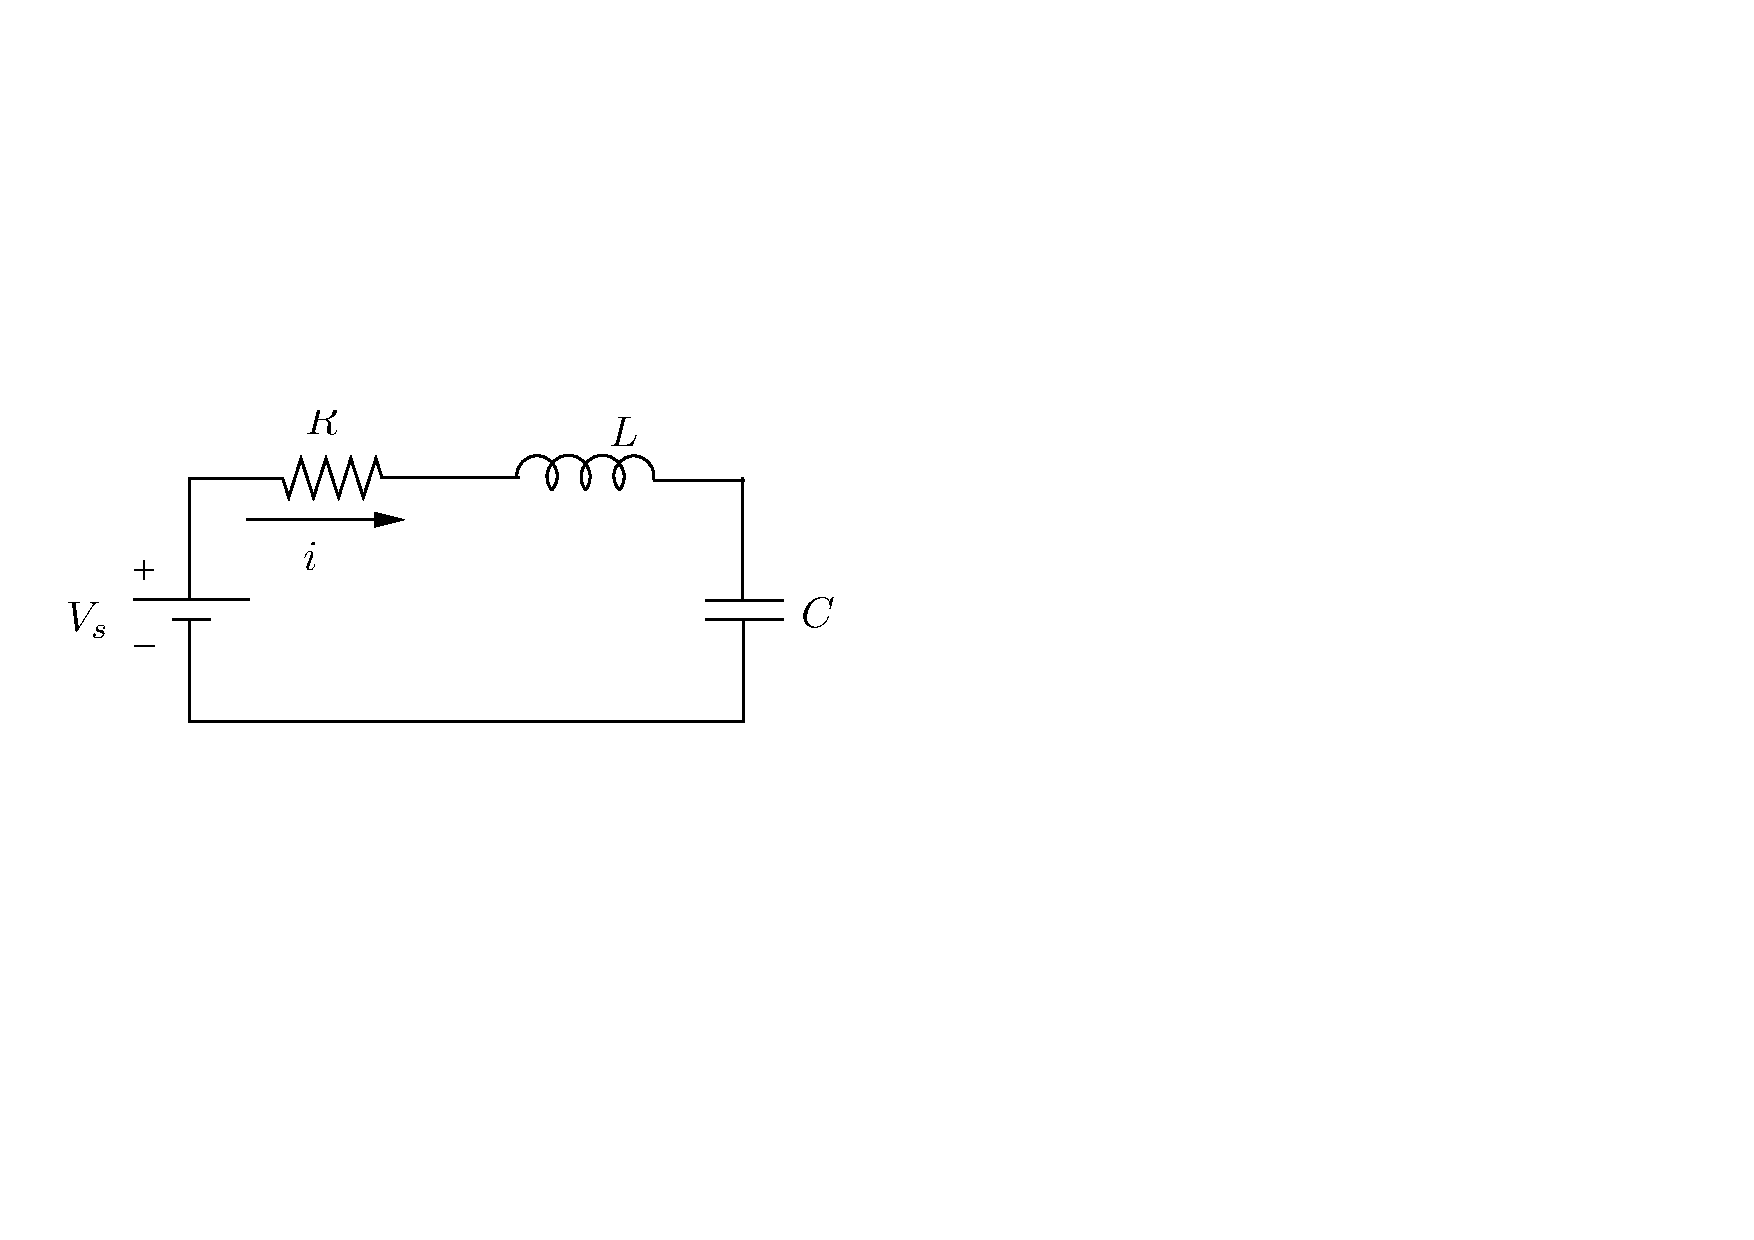
\includegraphics[width=1\linewidth]{images/RLC_serie}
	\end{column}
	\begin{column}{0.65\textwidth}
		\[L\frac{di}{dt}+R\, i+\frac{1}{C}\int_0^t i\, dx = V_s\]
		En dérivant :
		\begin{gather*}
		L\frac{d^2i}{dt^2}+R\frac{di}{dt}+\frac{1}{C} i = 0\\
		\frac{d^2i}{dt^2}+\frac{R}{L}\frac{di}{dt}+\frac{1}{LC} i = 0
		\end{gather*}
	\end{column}
	\end{columns}
	
	Même forme de solution pour le courant $i$ que dans le cas de la réponse libre.\\
	Dans les différentes expressions, remplacer $u_{C0}$ par $V_s$.
\end{frame}



\begin{frame}{Tensions aux bornes des éléments du circuit}
	
	\begin{align*}
	u_R(t) & =Ri(t) \quad \text{idem réponse libre avec $u_{C0}$ remplacé par $V_s$} \\
	u_L(t) & = L\frac{di}{dt} \quad \text{idem réponse libre avec $u_{C0}$ remplacé par $V_s$} \\
	u_C(t) & = V_s-u_R(t)-u_L(t)
	\end{align*}
	Dans le cas du régime oscillatoire amorti, on trouve :
	\[u_C(t)=V_s-\frac{\alpha V_s}{\omega_d}e^{-\alpha t}\sin \omega_d t - V_se^{-\alpha t}\cos \omega_d t\]
\end{frame}

%
%\section{Synthèse}
%\begin{frame}[allowframebreaks]{Synthèse}
%	
%	\vfill
%	
%	On considère des circuits comportant:
%	\begin{itemize}
%		\item[$\bullet$] des sources \textbf{indépendantes} d'énergie
%		\item[$\bullet$] des éléments \textbf{linéaires} et \textbf{invariants} : 
%		\begin{itemize}
%			\item R: dissipe, ne stocke aucune énergie
%			\item C, L: non-dissipatifs, emmagasinent une énergie: \\ \vspace{0.3 cm} \hspace{1 cm} $w_C = \frac{1}{2} C V^2, \hspace{0.5 cm} w_L = \frac{1}{2} L I^2$
%		\end{itemize} 
%	\end{itemize}
%	
%	\vspace{0.5 cm}
%	
%	On étudie les phénomènes \textbf{transitoires} résultant:
%	\begin{itemize}
%		\item[$\bullet$] d'une variation brusque des courants/tensions des sources \\ \hspace{0.5 cm} $\Rightarrow$ \textbf{Réponse forcée}
%		\item[$\bullet$] d'une restitution  de l'énergie emmagasinée (par C, L) \\ \hspace{0.5 cm} $\Rightarrow$ \textbf{Réponse libre}
%	\end{itemize}
%	
%	
%	Tension et courant dans un \textbf{condensateur}: 
%	
%	$$ v_c (t) = \frac{1}{C} \int_{-\infty}^{t} i_c(t') \: \mathrm{d}t' = v_c(0) + \frac{1}{C} \int_{0}^{t} i_c(t') \: \mathrm{d}t' \hspace{0.2 cm} \mbox{(continuité)}$$
%	$$\Leftrightarrow \hspace{0.3 cm} \boxed{i_c(t) = C \dfrac{\mathrm{d} v_c(t)}{\mathrm{d}t}} \hspace{0.3 cm} \Rightarrow [C] = s/\Omega \equiv \mbox{Farad}$$
%	
%	\vspace{0.5 cm}
%	
%	Tension et courant dans une \textbf{inductance}:
%	
%	$$ i_L(t) = \frac{1}{L} \int_{-\infty}^{t} v_L(t') \: \mathrm{d}t' = i_L(0) + \frac{1}{L} \int_{0}^{t} v_L(t') \: \mathrm{d}t' \hspace{0.2 cm} \mbox{(continuité)}$$
%	$$\Leftrightarrow \hspace{0.3 cm} \boxed{v_L(t) = L \dfrac{\mathrm{d} i_L(t)}{\mathrm{d}t}} \hspace{0.3 cm} \Rightarrow [L] = \Omega.s \equiv \mbox{Henry}$$
%	
%	
%	\begin{minipage}{0.4\textwidth}
%		Circuit \textbf{RC}: $\boxed{\tau = RC}$ 
%	\end{minipage}
%	\begin{minipage}{0.45\textwidth}
%		\begin{circuitikz}[european voltages]
%			\draw
%			(0,0)
%			to[american voltage source, l=$e(t)$, invert] ++(0,1.8)
%			to[R, l=$R$, i>=$i(t)$] ++(4,0) coordinate (A)
%			to[C, v^=$v_c(t)$] ++(0,-1.8)
%			--(0,0)
%			;
%		\end{circuitikz}
%	\end{minipage}
%	
%	\vfill
%	\begin{minipage}[l]{.48\linewidth}
%		\begin{center}
%			Réponse forcée \\ \vspace{0.3 cm}
%			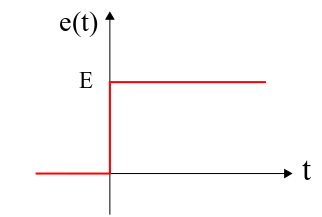
\includegraphics[scale=0.3]{images/echelon-tension1} \\
%			\hspace{1 cm} 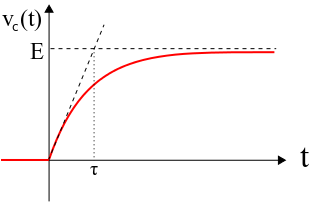
\includegraphics[scale=0.3]{images/charge-condensateur}
%		\end{center}
%	\end{minipage}
%	\begin{minipage}[l]{.48\linewidth}
%		\begin{center}
%			Réponse libre \\ \vspace{0.3 cm}
%			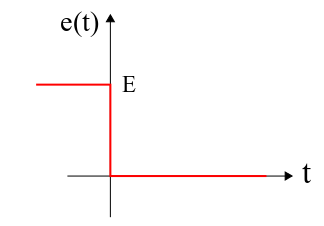
\includegraphics[scale=0.3]{images/echelon-tension2} \\
%			\hspace{0,9 cm} 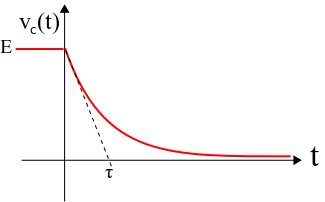
\includegraphics[scale=0.3]{images/decharge-condensateur}
%		\end{center}
%	\end{minipage}
%	
%	
%	
%	\begin{minipage}{0.4\textwidth}
%		Circuit \textbf{RL}: $\boxed{\tau = L/R}$  
%	\end{minipage}\begin{minipage}{0.45\textwidth}
%	\begin{circuitikz}[european voltages]
%		\draw
%		(0,0)
%		to[american voltage source, l=$e(t)$, invert] ++(0,1.8)
%		to[R, l=$R$, i>=$i_L(t)$] ++(4,0) coordinate (A)
%		to[L] ++(0,-1.8)
%		--(0,0)
%		;
%	\end{circuitikz}
%\end{minipage}
%	\vfill
%\begin{minipage}[l]{.48\linewidth}
%	\begin{center}
%		Réponse forcée \\ \vspace{0.3 cm}
%		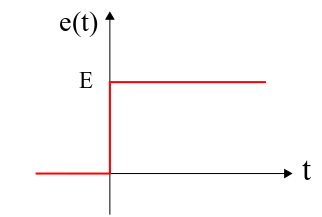
\includegraphics[scale=0.3]{images/echelon-tension1} \\
%		\hspace{1 cm} 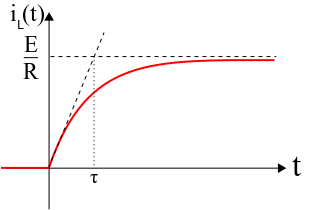
\includegraphics[scale=0.3]{images/etablissement-courant}
%	\end{center}
%\end{minipage}
%\begin{minipage}[l]{.48\linewidth}
%	\begin{center}
%		Réponse libre \\ \vspace{0.3 cm}
%		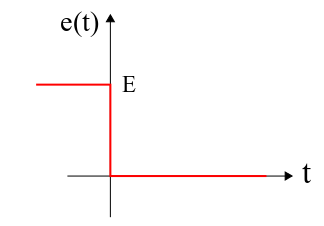
\includegraphics[scale=0.3]{images/echelon-tension2} \\
%		\hspace{0,8 cm} 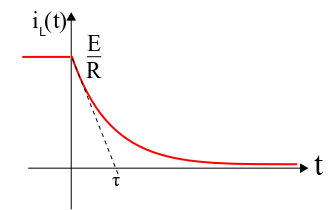
\includegraphics[scale=0.3]{images/rupture-courant}
%	\end{center}
%\end{minipage}
%
%	
%	Circuit \textbf{RLC série} initialement relaxé, source continue $V$ appliquée en $t=0$:
%	\begin{center}
%		$\boxed{\dfrac{\mathrm{d}^2 i(t)}{\mathrm{d}t^2} + \dfrac{R}{L} \dfrac{\mathrm{d} i(t)}{\mathrm{d}t} + \frac{1}{LC} i(t) = 0}\qquad   \alpha = \dfrac{R}{2L} \hspace{0.5 cm} \omega_0 = \dfrac{1}{\sqrt{LC}}$\\[5mm]
%		$s^2 + \frac{R}{L} s + \frac{1}{LC} = 0 \hspace{1 cm} \ \Rightarrow \ s_{1, \: 2} = - \alpha \pm \sqrt{\alpha^2 - \omega_0^2}$ 
%	\end{center}
%	\begin{minipage}[c]{.5\linewidth}
%		
%		\begin{itemize}
%			\item \textcolor{myRed}{$\alpha^2 - \omega_0^2 = \alpha_1^2> 0$} $\rightarrow$ Régime \textcolor{myRed}{apériodique}:
%			\begin{center}
%				\vspace{0.2 cm}
%				$i(t) = \frac{V}{\alpha_1 L} \: e^{- \alpha t} \: sinh(\alpha_1 t), \ t \geq 0$
%				\vspace{0.2 cm}
%			\end{center}
%			\item \textcolor{myRed}{$\alpha^2 - \omega_0^2 = 0$} $\rightarrow$ Régime \textcolor{myRed}{apériodique critique}
%			\begin{center}
%				\vspace{0.2 cm}
%				$i(t) = \frac{V}{L} \: t \: e^{- \alpha t}, \ t \geq 0$
%				\vspace{0.2 cm}
%			\end{center}
%			\item \textcolor{myRed}{$\alpha^2 - \omega_0^2 = - \omega_d^2 < 0$} $\rightarrow$ Régime \textcolor{myRed}{oscillatoire amorti}
%			\begin{center}
%				\vspace{0.2 cm}
%				$i(t) = \frac{V}{\omega_d L} \: e^{- \alpha t} \: sin(\omega_d t), \ t \geq 0$
%				\vspace{0.2 cm}
%			\end{center}
%		\end{itemize}
%	\end{minipage}
%	\begin{minipage}[l]{.15\linewidth}
%		\begin{center}
%			\begin{circuitikz}[european voltages]
%				\draw
%				(0,0)
%				to[american voltage source, l_=$V$, invert] ++(0,4)
%				to[short, i=$i$] ++ (1.5,0)
%				to[R, l=$R$] ++(0,-1.5) coordinate (A)
%				to[L, l=$L$] ++(0,-1.5)
%				to[C, l=$C$] ++(0,-1)
%				--(0,0)
%				;
%			\end{circuitikz}
%			%\includegraphics[scale=0.05]{RLC_series_circuit}
%		\end{center}
%	\end{minipage}
%		
%\end{frame}